% This is "sig-alternate.tex" V2.0 May 2012
% This file should be compiled with V2.5 of "sig-alternate.cls" May 2012
%
% This example file demonstrates the use of the 'sig-alternate.cls'
% V2.5 LaTeX2e document class file. It is for those submitting
% articles to ACM Conference Proceedings WHO DO NOT WISH TO
% STRICTLY ADHERE TO THE SIGS (PUBS-BOARD-ENDORSED) STYLE.
% The 'sig-alternate.cls' file will produce a similar-looking,
% albeit, 'tighter' paper resulting in, invariably, fewer pages.
%   
% ----------------------------------------------------------------------------------------------------------------
% This .tex file (and associated .cls V2.5) produces:
%       1) The Permission Statement
%       2) The Conference (location) Info information
%       3) The Copyright Line with ACM data
%       4) NO page numbers
%
% as against the acm_proc_article-sp.cls file which
% DOES NOT produce 1) thru' 3) above.
%
% Using 'sig-alternate.cls' you have control, however, from within
% the source .tex file, over both the CopyrightYear
% (defaulted to 200X) and the ACM Copyright Data
% (defaulted to X-XXXXX-XX-X/XX/XX).
% e.g.
% \CopyrightYear{2007} will cause 2007 to appear in the copyright line.
% \crdata{0-12345-67-8/90/12} will cause 0-12345-67-8/90/12 to appear in the copyright line.
%
% ---------------------------------------------------------------------------------------------------------------
% This .tex source is an example which *does* use
% the .bib file (from which the .bbl file % is produced).
% REMEMBER HOWEVER: After having produced the .bbl file,
% and prior to final submission, you *NEED* to 'insert'
% your .bbl file into your source .tex file so as to provide
% ONE 'self-contained' source file.
%
% ================= IF YOU HAVE QUESTIONS =======================
% Questions regarding the SIGS styles, SIGS policies and
% procedures, Conferences etc. should be sent to
% Adrienne Griscti (griscti@acm.org)
%
% Technical questions _only_ to
% Gerald Murray (murray@hq.acm.org)
% ===============================================================
%
% For tracking purposes - this is V2.0 - May 2012

\documentclass{sig-alternate}

\usepackage[lined,ruled,linesnumbered,vlined]{algorithm2e}
\usepackage{epstopdf}
\usepackage{color}

\usepackage{tikz}

\usepackage{multirow}
\usepackage{graphicx}
\usepackage{psfig}
\usepackage{pgfplots}
%\usepackage{subcaption}
\usepackage{syntax}
\usepackage{url}
\usepackage{subfigure}
\usepackage{balance} 
\usepackage{colortbl}
\usepackage{booktabs}
\usepackage{subfig}

% %\usepackage{amsthm}

%%%%%%%%%%%%%%%%%%%%%%
% the following is to handle the incompatibility between syntax and source-compilation.
%%%%%%%%%%%%%%%%%%%%%%
\makeatletter
\def\gr@implitem#1<#2> #3 {%
\sbox\z@{\hskip\labelsep\grammarlabel{#2}{#3}}%
\strut\@@par%
\vskip-\parskip%
\vskip-\baselineskip%
\hrule\@height\z@\@depth\z@\relax%
\item[\unhbox\z@]%
\catcode`\<\active%
}
\makeatother


\newtheorem{theorem}{Theorem}
\newtheorem{definition}{Definition}
\newtheorem{lemma}{Lemma}
\newtheorem{example}{Example}
\newtheorem{corollary}{Corollary}
\newcommand{\TODO}[1]{\textcolor{red}{\textbf{TODO:} \{#1\}}}


\begin{document}
%
% --- Author Metadata here ---
\conferenceinfo{SIGKDD}{'16 San Francisco, California USA}
\CopyrightYear{2016} % Allows default copyright year (20XX) to be over-ridden - IF NEED BE.
%\crdata{0-12345-67-8/90/01}  % Allows default copyright data (0-89791-88-6/97/05) to be over-ridden - IF NEED BE.
% --- End of Author Metadata ---

\title{Scalable Correlating Heterogeneous Time Series}
 
%\subtitle{[Extended Abstract]
%\titlenote{A full version of this paper is available as
%\textit{Author's Guide to Preparing ACM SIG Proceedings Using
%\LaTeX$2_\epsilon$\ and BibTeX} at
%\texttt{www.acm.org/eaddress.htm}}}

%
% You need the command \numberofauthors to handle the 'placement
% and alignment' of the authors beneath the title.
%
% For aesthetic reasons, we recommend 'three authors at a time'
% i.e. three 'name/affiliation blocks' be placed beneath the title.
%
% NOTE: You are NOT restricted in how many 'rows' of
% "name/affiliations" may appear. We just ask that you restrict
% the number of 'columns' to three.
%
% Because of the available 'opening page real-estate'
% we ask you to refrain from putting more than six authors
% (two rows with three columns) beneath the article title.
% More than six makes the first-page appear very cluttered indeed.
%
% Use the \alignauthor commands to handle the names
% and affiliations for an 'aesthetic maximum' of six authors.
% Add names, affiliations, addresses for
% the seventh etc. author(s) as the argument for the
% \additionalauthors command.
% These 'additional authors' will be output/set for you
% without further effort on your part as the last section in
% the body of your article BEFORE References or any Appendices.

\numberofauthors{2} %  in this sample file, there are a *total*
% of EIGHT authors. SIX appear on the 'first-page' (for formatting
% reasons) and the remaining two appear in the \additionalauthors section.
%
\author{
% You can go ahead and credit any number of authors here,
% e.g. one 'row of three' or two rows (consisting of one row of three
% and a second row of one, two or three).
%
% The command \alignauthor (no curly braces needed) should
% precede each author name, affiliation/snail-mail address and
% e-mail address. Additionally, tag each line of
% affiliation/address with \affaddr, and tag the
% e-mail address with \email.
%
% 1st. author
\alignauthor
Chen Luo\\
	   \affaddr{Department of Computer Science}\\
       \affaddr{Rice University}\\
       %\affaddr{No. 2699 Qianjin Street}\\
       \affaddr{Houston, TX, USA}\\
       \email{cl67@rice.edu}
% 2nd. author
\alignauthor
Anshumali Shrivastava\\
	   \affaddr{Department of Computer Science}\\
       \affaddr{Rice University}\\
       %\affaddr{No. 2699 Qianjin Street}\\
       \affaddr{Houston, TX, USA}\\
       \email{anshumali@rice.edu}
}
% There's nothing stopping you putting the seventh, eighth, etc.
% author on the opening page (as the 'third row') but we ask,
% for aesthetic reasons that you place these 'additional authors'
% in the \additional authors block, viz.

%\date{30 July 1999}

% Just remember to make sure that the TOTAL number of authors
% is the number that will appear on the first page PLUS the
% number that will appear in the \additionalauthors section.

\maketitle

\begin{abstract}

%Calculating the correlation between different time series is an important data mining task. 
%In recent years, time series data have two major properties: (1) Heterogeneity property (Different Time series may have different patterns.) and (2) High Dimensional and Large Scale. 
%In addition, for heterogeneous time series with different pattern, they may also have high correlation. Despite their importance, there has been little previous work addressing the correlation between two types of heterogeneous time series data.
%
%In this paper, we propose an approach that is capable of (1) evaluating evaluate the correlation between heterogeneous time series (time series with different patterns), and (2) dealing with very large scale problems.
%We investigated a change based correlation Coefficient to evaluate the correlation between different heterogeneous time series. In addition, we proposed hashing based method to do fast searching and clustering on very large scale time series.
%The experimental results on Synthetic data sets and real world data set show
%the effectiveness and efficiency of our algorithms.

\end{abstract}
% A category with the (minimum) three required fields
\category{H.2.8}{Database Management}{Data Mining}

\terms{Application}

\keywords{Correlation, Time Series, Hashing Learning}

\section{Introduction}
\label{sec:introduction}

\begin{figure}[t]
\centering
\includegraphics[width=0.5\textwidth]{ECGExp.eps}
\caption{ Five ECG time-series corresponding to three different diseases. Different color denotes different diseases.}
\label{fig:ecgexample}
\end{figure}

\begin{figure}[t]
\centering
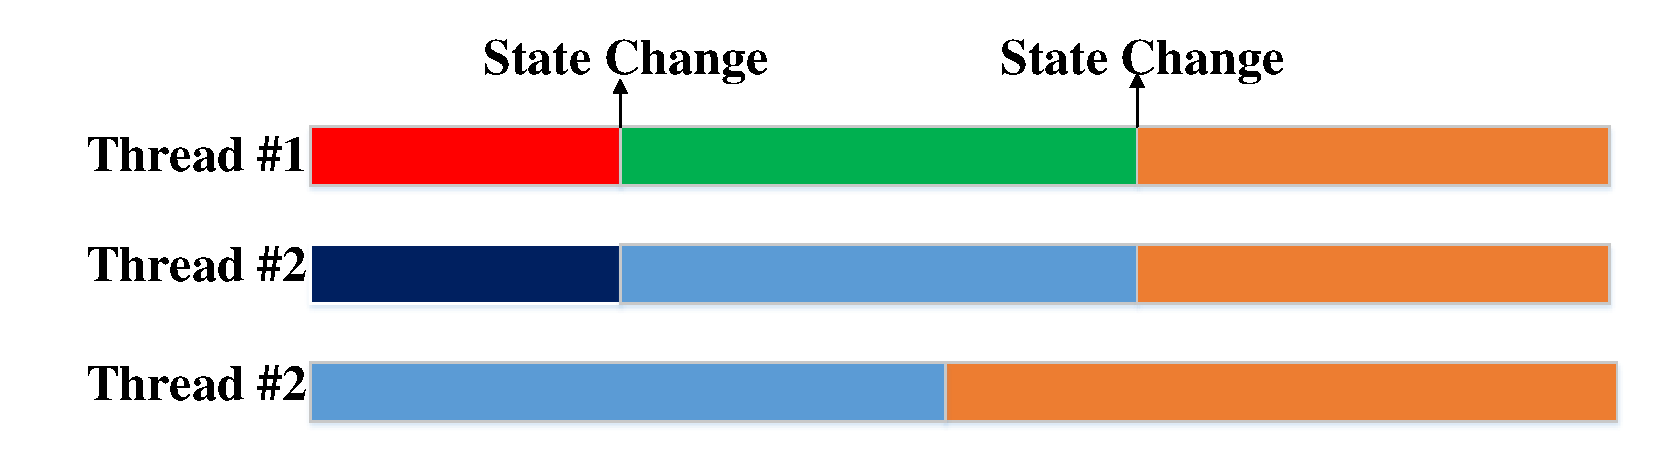
\includegraphics[width=0.50\textwidth]{HPCExample.pdf}
\caption{Snapshot of HPCToolket Traceviewer of an environment simulation task.
Each line represent one thread, \textbf{Thread0} to \textbf{Thread3} belongs to a Ocean Simulation Program, and \textbf{Thread4} to \textbf{Thread8} belongs to a Weather Simulation Program. Different Color in each thread denotes the ``Call Path" state.}
\label{fig:hpcexample}
\end{figure}

The focus of this paper will be on the time series data. A time series is defined as a sequence of values $\{s_1,s_2,...,s_m\}$
associated with timestamps $\{t(s_1), t(s_2),..., t(s_m)\}$, which typically has the relationship of $t(s_i) = t(s_{i-1})+\tau$, where $\tau$ is  the sampling interval, and $m$ is the number of points in the time series.

Time series mining is ubiquitous in data driven applications including robotics, medicine~\cite{oates2000method,caracca2000discovering}, speech~\cite{rabiner1993fundamentals}, object detection in vision~\cite{yang2002detecting, sonka2014image}, High Performance Computing (HPC) and system failure diagnosis~\cite{luo2014correlating,sun2014querying}, Earth Science \cite{mudelsee2013climate}, Finance \cite{granger2014forecasting}, etc.

Due to its pervasive presence, time series mining have received significant attention in recent years. A common prerequisite for data mining algorithms, such as clustering, search, classification and regression, etc., is a measure of correlation (or similarity). Dynamic Time Warping (DTW) is widely accepted, and arguably the most popular, measure of similarity (or correlation) for time series data in general~\cite{rakthanmanon2012searching, muller2007dynamic, chen2013dtw}.

All existing measures over time series, including the popular DTW, relies on the notion that two time series $S_1$ and $S_2$ are similar, if there is a long enough, similarly behaving, subsequence common between them. This is a very reasonable notion which is also the desired nature of the similarity function in many applications.  However, there are plenty of real-world problems where the similarity of interest has a very different notion. Despite their importance, there has been little previous work addressing such scenarios. To signify their importance, we provide two motivating real-world examples:


\textbf{ECG (Electrocardiogram) data}

Electrocardiography \cite{holter1961new} (ECG or EKG*) generates time series data, where each time series is the electrical activity of the heart over a period of time. This activity is measured using electrodes placed on a patient's body, which detect the tiny electrical changes on the skin that arise from the depolarization of the heart muscle during each heartbeat. The tiny electrical changes occurs in different rhythm corresponds to different heart physical states or different diseases. This depolarization  if usually different for different patient. The characteristic of a disease is typically the time of sudden change in the electrical signal, i.e., if two ECG often have tiny electrical changes at the same time, they indicate same disease or same heart physical state~\cite{marriott1988practical}.

%,

As an illustration, Fig. \ref{fig:ecgexample} shows five ECG time series from a real data ({\bf Give description}). These five ECG comes from three different diseases denoted by color green, blue and red.  The DTW distance between ECG1 and ECG2 is $0.2$, while the distance between ECG2 and ECG3 is $0.5$. This is clearly not correct. Time series corresponding to same disease, for this ECG data, should have closer distance compared to time series corresponding to different diseases. 

It is not surprising that we should not use the traditional measure of similarity for this task. This because that the similarity of ECG time series data correspond to the change rhythm, not correspond to the point to point similarity as evident from the Figure~\ref{fig:ecgexample}.
Since the ECG time series data have different change patterns (e.g. Increase-Decrease, Decrease-Increase, or a Sudden wave, etc.). These different change patterns can effect the performance of point to point similarity measures.

On the other hand, By using the similarity in this work, the correlation between ECG1 and ECG2 is $1.00$, and the similarity between ECG1 and ECG3 is $0.25$, which clearly agrees with the gold standard labels.

%

%We choose three time series from two different labels in that data set.
%We illustrate this in Figure\ref{fig:ecgexample}, where we show the hierarchical clustering of these three time series under various measures.
%Top two red bold time series ($ECG\#1,ECG\#2$) are labeled as same class, and $ECG \#3$ is labeled as other class.




%correlation is a major research topic in data mining area.
%Such correlating techniques has been applied in many real world problems.
%For example, some researchers use time series correlation techniques to analysis the signal information for speech processing \cite{rabiner1993fundamentals}.
%Image processing researchers also use time series correlation techniques to deal with the image retrieval problems and object detection problems \cite{yang2002detecting, sonka2014image}.
%In the system diagnose area\cite{luo2014correlating,sun2014querying}, time series correlation techniques also widely used to mine the system behavior and diagnose system failures.
%Time series correlation techniques can also be used for analyzing bio-sequences (e.g DNA Sequence, etc \cite{mount2001bioinformatics} etc.

%In addition, real world time series are all high dimensional and large scale data, how to mining such huge amount of data set is also a challenge for us.
%By analyzing such data, one can find some useful information hidden behind the human body, thus to uncover some miracles of human body \cite{tilley1979essentials}.
%The first real-world example is ECG data\cite{holter1961new}.


\textbf{High-Performance Computing (HPC) Logs:} High-performance computers (HPC) have become enormously complex. Today, the largest systems consist of more than tens of thousands of nodes. Nodes themselves are equipped with one or more multicore microprocessors\cite{adhianto2010hpctoolkit}. High-performance computer can generate over billions of threads during running.
Automatically analysing and monitoring the HPC has recently grabbed significant attention by the HPC researchers \cite{mccurdy2010memphis,tallent2009effective}.

%As a result, it is increasingly difficult for application developers writing complex scientific programs to attain a significant fraction of peak performance on modern microprocessor-based computer systems.

HPCToolkit\footnote{http://hpctoolkit.org/} can be used to profile different threads from High performance computers.
Information from each thread can be represented as a time series. The value of the time series denote the call path \cite{adhianto2010hpctoolkit} state of the thread.

%(Depend on which aspect of a thread to be represent, domain knowledge required) The thread change information (e.g. change from one state to another state) can directly reflect some important properties of different threads.

Fig. \ref{fig:hpcexample} shows a example of nine thread time series data coming from {\bf where does it come from}. Different colors means different call path state. Here, \textbf{Thread0} to \textbf{Thread3} belongs to a Ocean Simulation Program, and \textbf{Thread4} to \textbf{Thread8} belongs to a Weather Simulation Program. Different Color in each thread denotes the ``Call Path" state.

It is obvious that threads from the same program are highly correlated. This correlation can be detected by the existing method such as Pearson correlation or DTW distance. For example, the DTW distance between Thread 0 and Thread 1 is $0.05$, which denotes they are highly correlated.

However, for the Environment Simulation Task, Ocean simulation Program and Weather Simulation Program are also correlated with each other. Because in the real world, the weather earth are correlated with the activities of the ocean.  So these two programs often change data during simulating, when they change data, they will change state at the same time.

And this type of correlation (Threads Correlation between Different Programs) can not be detected using DTW distance. For example, the DTW distance between Thread 0 and Thread 4 is $0.8$. While using our method, we can find a $0.6$ correlation coefficient with each other.

We can see that DTW and Euclidean distance can not perform well. Because threads in the different program always have different states and DTW and Euclidean will regard these state difference as large distance.
On the other hand, change based correlation only consider the change information of the time series, and the state difference between different threads of each program can not bias the correlation result.


%However, in most real world problems, time series data often have different patterns (Heterogeneous time series). For example, in the area of system analysis area.
%Each performance counter can be regarded as a time series (e.g. CPU Usage, Memory Usage, etc.).
%Some of the time series may be a periodical time series, but others may be a linear or random patterns.
%However, heterogeneous time series may also be correlations between each other.
%So, how to calculate the correlation between heterogeneous time series data is a challenge.

As showed in above examples, the existing point to point time series similarity measures (e.g. L1-Distance, L2-Distance \cite{han2011data}, and DTW-Distance \cite{muller2007dynamic}, etc) or correlation measures (e.g. Pearson Correlation \cite{pearson1904mathematical}, Kendall rank correlation \cite{kendall1938new}, and Spearman's rank correlation \cite{pirie1988spearman}, etc.) can not deal with time series similarity problem when time series have heterogeneous patterns.
The reason is: for heterogeneous time series, the correlation information is often associated with the change (During a period of time) of time series, rather than a point-to-point relationship in the traditional correlation analysis techniques. We will introduce the related research of point to point based similarity measure in detail in Section \ref{sec:relatedwork}.

As a result, in order to deal with heterogeneity properties of time series, we proposed a change based correlation coefficient.
Our change based correlation method firstly extract the change information of the time series data, and then use the change information to calculate the correlation coefficient between the two time series.
By taking the advantage of this correlation coefficient, we propose to use LSH method to dealing with very large top-k searching problems.

The contribution of this paper is listed as follow:
\begin{enumerate}
\item Motivated by real applications, we investigate the correlation
problem as between heterogeneous time series .
To the best of our knowledge, this is the first attempt
to evaluate the correlation between time series with different patterns.

\item We proposed a correlation coefficient between heterogeneous time series. By taking the advantage of this correlation coefficient, we can do searching and mining on large scale time series datasets.


\item The experiments on Synthetic data sets and Real world data sets show the effectiveness and efficiency of our method.
\end{enumerate}

The rest of the paper is organized as follows: In Section 2, we introduce the problem
statement and formulation. Our approach is proposed in Section 3. The Empirical evaluation is shown in Section 4. In Section 5, we introduce some
related works. Finally, we conclude our work in Section 6.





\section{Background}
\label{sec:formulation}

\subsection{Preliminary Definition}

In this section, we formally define some concept of this work, including Time Series, Change Point, Change Point set, Time Series Correlation.

\begin{definition}[Time Series]
A time series, denoted as $S = (s_1,s_2,...,s_m)$, where $m$ is the number of points in the time series. The timestamps of a time series, denoted as $TS = (t(s1), t(s2),..., t(sn))$, have the relationship of $t(s_i) = t(s_{i-1})+\tau$, where $\tau$is the sampling interval.
\end{definition}

In this work, we consider the change information of a time series, so the change point of a time series is defined as follow:
\begin{definition}[Change Point]
A time series, denoted as $S = (s_1,s_2,...,s_m)$, a change point is a time stamp $t_s(i)$that there is a change before and after this time stamp. Change contains the following types: mean change, variance change,  frequency change, and the combination between them.
\end{definition}

The definition of change point set is defined as follow:
\begin{definition}[Change Point Set]
A time series, denoted as
$S = (s_1,s_2,...,s_m)$
The timestamps of a time series, denoted as 
$TS = (t(s1), t(s2),..., t(sn))$
The change points set is denoted as 
$C_X=(t_x(1),t_x(2),...,t_x(p))$
Where $t_x(i)$ denotes the change points of time series S.
\end{definition}


\subsection{Change based Time Series Correlation}

After define the time series, we define the correlation of this work as follow:
\begin{definition}[Change Based Correlation] 
Suppose we have two time series: $X_1=(x_1,x_2,...,x_m),Y_1=(y_1,y_2,...,y_m)$, The change point set of X and Y are denoted as: 
$C_X=(t_x(1),t_x(2),...,t_x(p))$
$C_Y=(t_y(1),t_y(2),...,t_y(q))$
where $q$ and $p$ are numbers of change points for time series $X$ and $Y$.
Then if $X$ and $Y$ are correlated if and only if:
\begin{equation}
\left\{\begin{matrix}
p=q\\ 
L1(C_X,C_Y)<\xi 
\end{matrix}\right.
\end{equation}
where $L1(C_X,C_Y)$ denotes the L1 distance, and $\xi$ is the threshold of Time series correlation.
\end{definition}


\section{The Approach}
\label{sec:framework}
In this section, we first propose a framework to analyze the correlation of heterogeneous time series, and then we introduce how to use hashing method to do fast searching.

\subsection{Change Based Correlation Coefficient}

The Change Based Correlation Coefficient can be calculated following the framework in Fig. \ref{fig:frame}.
Given a time series, first, we extract the change information of the time series. 
In this work, we regard the change information as bit-stream. In the bit-stream, $1$ denotes there is a change in this sub-series, and $0$ if not. We will introduce the change based information in details in the following section.

After obtaining the change information of the time series, we then calculate the Jaccard similarity\cite{han2011data} coefficient between each other.
As we defined before (Section \ref{sec:formulation}), if two time series often change at the same time, they may have correlation with each other. 
So, here, how often denotes the value of the correlation. In other words, how many $1$ do two time series both have. This is directly the Jaccard Distance.
So, the Jaccard similarity between each bit-stream will be the correlation coefficient between these two time series. 

\begin{figure}[t]
\centering
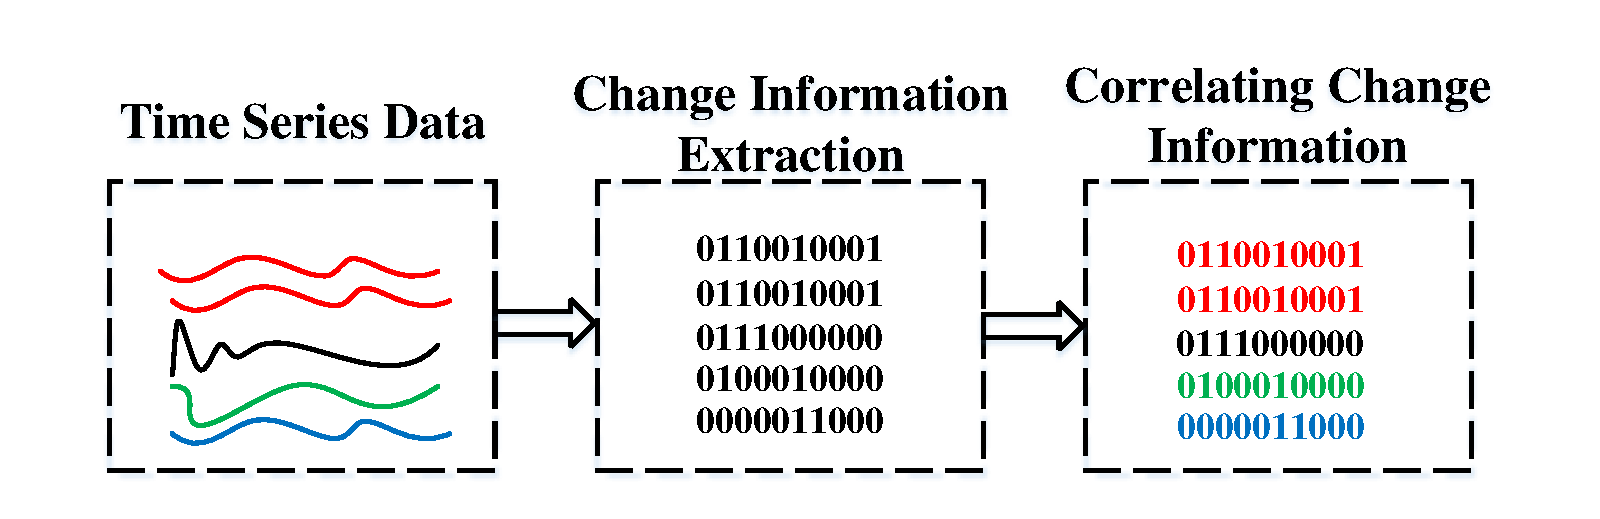
\includegraphics[width=0.5\textwidth]{framework.pdf}
\caption{Overview of the Framework}
\label{fig:frame}
\end{figure}

\subsection{Change Information Extraction}
\label{ChangeCorrelation}

As we introduced in Section.\ref{sec:formulation}, change based correlation corresponds to the change information of the time series. change information of a time series is a time period information, not a time point information. 
As a result, in order to extract the change information of the time series, we need to find the information in small time period of the time series (A sub-series). The idea of extracting the change information is showed in Fig.\ref{fig:ChangeMapping}.

Given a time series $S = (s_1,s_2,...,s_m)$, where $m$ is the number of points in the time series. Given a subs-series length $k$. The change information of the time series $S$ can be represented as a bit-stream:

$B_S = \{b_0,b_1,...,b_n\}$, where each $b_i$ corresponds to a sub-series of length $k$ for the original time series $S$ as showed in 

Given a sub-series $l^j = \{s_i,s_{i+1},s_{i+2},...,s_{i+k-1}\}$, where $w$ is the length of the sub-series. Then the change information of sub-series $l$ is denoted as follow:

\begin{equation}
\label{Equ:ChangeInformation}
b^l = \left\{\begin{matrix}
1 & Have~change~in~l
\\ 
0 & No~change~in~l
\end{matrix}\right.
\end{equation}

\begin{figure}[t]
\centering
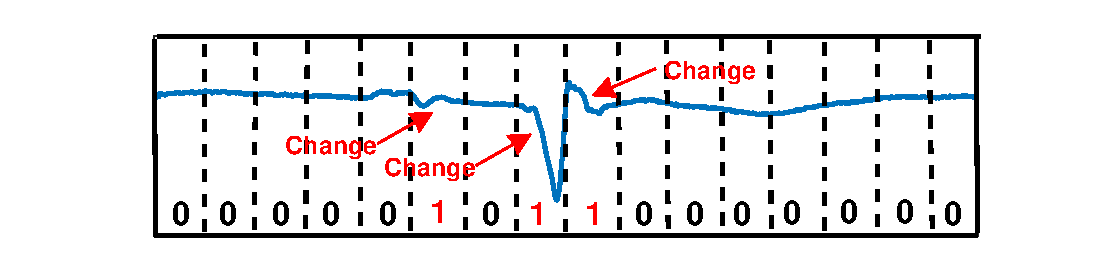
\includegraphics[width=0.5\textwidth]{changeExtraction.eps}
\caption{Change Information Extraction}
\label{fig:ChangeMapping}
\end{figure}

As showed in Equ.\ref{Equ:ChangeInformation}, the change information is the information that whether there's a change in the sub-series. In order to denote whether there's a change in the sub-series, we need to know to to detect change in the sub-series.
Fig.\ref{fig:ChangeMapping} shows how to extract the change information of the time series.

\subsection{Change Detection}
\label{sec:changeDetect}
So,the problem here is:
Given a sub-series 

$l^j = \{s_i,s_{i+1},s_{i+2},...,s_{i+k-1}\}$, 

how to denote whether there is a change or not in this time series.
There are a so many time series change detection methods \cite{liu2013change,chen2013contextual} proposed in the literature. 

In this work, the change detection task here is not find the change points of the time series, instead we only need to denote whether there's a change in the time series. It is pointed out that all the change point detection methods can be used here to detect change information.
In our experiment, we use the the following method to detect change:

We equally divide the time series into two series: 

$l^j_{Front} = \{s_i,s_{i+1},s_{i+2},...,s_{i+(k-1)/2 -1}\}$

and, 

$l^j_{Front} = \{s_{i+(k-1)/2 -1},s_{i+(k-1)/2},...,s_{i+k-1}\}$.

So, regard $l^j_{Front}$ and $l^j_{Rear}$ as two data sampled from two distributions $P_1$ and $P_2$. So, if $P_1$ and $P_2$ are statistically the same, then we can say there's not change between each other. Otherwise, there is a change in this dataset.

Then, the problem here becomes a \textit{Two Sample Problem} \cite{gretton2006kernel}. We use the Two Sample \textit{t}-test \cite{moore2007basic} method to solve this problem:

Here, the $t_{score}$ between $l^j_{Front}$ and $l^j_{Rear}$ can be calculated as:

\begin{equation}
t_{score} = \frac{\overline{l^j_{Front}} - \overline{l^j_{Rear}}}{\sigma_p\sqrt{2/k}}
\end{equation}

where, $\overline{l^j_{Front}}$ and $\overline{l^j_{Front}}$ are the mean values of $l^j_{Front}$ and $l^j_{Front}$. And $\sigma_p$ is as follow:

\begin{equation}
\sigma_p = \frac{(k-1)\sigma_{l^j_{Front}}^2 + (k-1)\sigma_{l^j_{Rear}}^2}{k-1}
\end{equation}

Then, if $t_{score} > \alpha$, we can say that these two samples are from different distributions, and thus there is a change in the sub-series $l^j$.

\subsection{Jaccard Similarity Coefficient}

After obtaining the change information (Bit-stream) of each data, we then use Jacord Similarity Coefficient to calculate the Change Correlation of each time series.

The Jaccard Similarity \cite{han2011data} is defined as follow:
Given two Bit-stream $X$ and $Y$, the Jaccord distance is showed as follow:

\begin{equation}
J(A,B) = \frac{|A \cap B|}{|A \cup B|}
\end{equation}

where, $|A \cap B|$ denotes the number of bit that $X$ and $Y$ both $1$. And $|A \cup B|$ denotes the number of bit that at least $X$ or $Y$ is $1$.
For example, given two bit stream: $X={100111}$, and $Y={001110}$. Then $|A \cap B| = 2$, and $|A \cap B| = 5$, so $J(A,B) = \frac{2}{5} = 0.4$.


\subsection{Speed up Top-k Search using LSH}

In many the real world problems, the scale of time series data often huge \cite{rakthanmanon2012searching}. Mining such huge number of time series is a big challenge for us.

In this work, by taking the advantage of the change based coefficient, we propose to use Locality Sensitive Hashing to do large scale search in time series data.

The change information of a time series is a bit-stream (Section \ref{sec:changeDetect}). We regard it as the hashing code of the original time series.

As ar result, we can directly use LSH (Locality Sensitive Hashing) search algorithm to speed up the searching process. \cite{indyk1998approximate} 

\subsection{Discuss about Sub-series Length w}

In this research, the sub-series length $w$ is a very important parameter.
If the sub-series length $w$ is too short, then the change information can not be captured. 
On the other hand, if the sub-series length $w$ is too long, then there will be too much noise information.

In some cases, the value of $m$ can be selected based on domain knowledge and experiments. In the experiment of this work, all the sub-series length are selected based on the domain knowledge.

However, in most real world situations, there are millions of time series and events, and we do not have enough domain knowledge to pre-select the values of all sub-series lengths. 

In our previous research of Correlating Event with time series \cite{luo2014correlating}, we can auto-select the sub-series length for a time series based on the autocorrelation function \cite{hamilton1994time} of the time series.
Given a time series $S=(s_1,s_2,...,s_n)$, the autocorrelation is showed as follow:

\begin{equation}
R(l) = E(s_i*s_{i-l}).
\end{equation}
where $l$ denotes the lag of the correlation. The autocorrelation function of a time series can be used to represent the energy of signals in the time series with a period of $l$ \cite{hamilton1994time}. Therefore, our length $m$ can be assigned as the value of the first peak to include the significant signal of the time series. For more detail of this selection method, please refer \cite{luo2014correlating}.


\section{Empirical Evaluation}
In this section, we make an empirical evaluation of our algorithm by performing a set of experiments on the synthetic data set, and several real world data sets.

\subsection{Comparison Methods}
In order to evaluate the effectiveness of our algorithm, we choose three time series similarity algorithms and four correlation coefficient in our experiment. 

For the three similarity algorithm, we choose L1-Distance, L2-Distance \cite{han2011data}, and DTW-Distance \cite{muller2007dynamic}. 
And for the three similarity algorithm, we choose Pearson correlation \cite{nagelkerke1991note}, which is the widely used methods for correlation mining in time series. And also two ranking based correlation: The Kendall rank correlation \cite{kendall1938new}, and Spearman's rank correlation \cite{pirie1988spearman}.

In the rest of this subsection, we briefly introduce the three similarity measures and the three Correlation measures.
 
\subsubsection{Similarity Measures}

Given a two time series 
$X=(x_1,x_2,...,x_m),Y=(y_1,y_2,...,y_m)$.

The L1-distance is denoted as follow:

\begin{equation}
L1(X,Y) = \sum_{1}^{m}|x_i-y_i|
\end{equation}

The L2-distance is denoted as follow:

\begin{equation}
L1(X,Y) = \sqrt{\sum_{1}^{m}|x_i-y_i|^2}
\end{equation}

The third similarity measure we used is DTW distance \cite{muller2007dynamic}, which is a famous time series similarity measure.

In order to introduce the DTW distance, we firstly construct an $m-by-m$ matrix $W$, where the $(i-{th},j-{th})$ element of the matrix $W$. The DTW distance is to find a path through the matrix that minimizes the total cumulative distance between $X$ and $Y$. 
So, the optimal path is the path that minimize the warping cost:

\begin{equation}
DTW(X,Y) = \min { \sqrt{\sum_{k=1}^{K}w_k}}
\end{equation}
where, $w_k$ belongs to the $k-{th}$ element of a warping path $P$, which is a contiguous set of elements that represent a mapping between $X$ and $Y$.

\subsubsection{Correlation Measures}

In this subsection, we introduce three widely used correlation measures between time series: Pearson Correlation \cite{pearson1904mathematical}, Kendall rank correlation \cite{kendall1938new}, and Spearman's rank correlation \cite{pirie1988spearman}.

The Pearson correlation method is one of the most widely used method for measuring the correlation between two time series. The Pearson correlation coefficient, denoted as $\rho$. can be calculated as follow:

\begin{equation*}
\rho_{X,Y}^{Pearson}=\frac{cov(X,Y)}{\sigma_X\sigma_Y}=\frac{E[(X-\mu_X)(Y-\mu_Y)]}{\sigma_X\sigma_Y}
\end{equation*}
where $cov$ is the covariance, $\sigma_X$ is the standard deviation of $X$, $\mu_X$ is the mean of $X$ and $E[*]$ denotes the expectation.

The Kendall rank correlation \cite{kendall1938new} is defined as follow:

\begin{equation*}
\rho_{X,Y}^{Kendall}=\frac{N_c - N_d}{m(m-1)/2}
\end{equation*}

Where $N_c$ is the number of concordant pairs, and $N_d$ is the number of discordant pairs, and $m$ is the dimension of the time series.
For any pair $(x_i,y_i)$ and $x_j,y_j$, where $i \neq j$, are said to be concordant both $x_i > x_j$ and $y_i > y_j$, or $x_i < x_j$ and $y_i < y_j$. Otherwise, they are discordant.

The Spearman's rank correlation \cite{pirie1988spearman} is defined as follow:

\begin{equation*}
\rho_{X,Y}^{Spearman}=1 - \frac{6\sum d^2_i}{n(n^2-1)}
\end{equation*}

where $d_i$ is defined as the difference between the ranks of $x_i$ and $y_i$.

\subsection{Effectiveness Study on Synthetic Dataset}

In this section, we introduce the experiment on the synthetic Dataset.

\subsubsection{The Synthetic Dataset}

Synthetic data set is very useful for evaluating algorithms and functions for data mining and machine learning models\cite{han2011data}. 
In this section, we introduce the Synthetic Dataset used in our experiment.

In this synthetic Dataset, we randomly generate $10000$ time series with two patterns of time series: (1) Periodical Pattern, (2) Linear Pattern.
Each time series was added with white noise \cite{han2011data}. 
Then, we separate the $10000$ time series into five groups. And within each group, we add change randomly at the same time. (In each group, the change points are same.)
Seven different types of changes are added randomly into each time series, the seven change types are showed in Table.\ref{Tab:ChangeType}.

\begin{table}[t]
\caption{\textbf{Change Types in the Synthetic Data}}
\centering

\begin{tabular}{|c|}
\hline Change Type \\
\hline Mean Change \\
\hline Variance Change\\
\hline Frequency Change $+$ Variance Change\\
\hline Mean Change $+$ Frequency Change \\
\hline Frequency Change $+$ Variance Change\\
\hline Mean Change $+$ Frequency Change $+$ Variance Change\\
\hline
\end{tabular}
\label{Tab:ChangeType}
\end{table}

In order to test both the efficiency and effectiveness of change based correlation coefficient. We choose four sub-set from such dataset. 
We make the data set size from small to large, and also the time series length from short to long. The four sub dataset is showed in Table.\ref{Tab:SDataScale}. 

\begin{table*}
\caption{Clustering Performance on Synthetic Data Set}
\centering
\renewcommand{\arraystretch}{1.2}
\begin{tabular}{ccccccccc} 
\toprule[2pt] 
%\hline
Dataset & Measure & Proposed & $L1$ & $L2$ & DTW & Pearson & Kendall & Spearman \\
\toprule[1.5pt] 
\multirow{2}*{\centering{Sythetic-T0}}
     & Accuracy & $\boldsymbol{.854\pm.032}$ & $.241\pm.098$ & $.281\pm.012$ & $.230\pm.061$ & $.309\pm.140$ & $.353\pm.026$ & $.297\pm.036$ \\
\cline{2-9}
     & NMI & $\boldsymbol{.808\pm.034}$ & $.026\pm.067$ & $.076\pm.023$ & $.028\pm.075$ & $.140\pm.55$ & $.395\pm.015$ & $.150\pm.088$ \\
\toprule[1.2pt] 
\multirow{2}*{\centering{Sythetic-T1}}
     & Accuracy & $\boldsymbol{.838\pm.025}$ & $.247\pm.026$ & $.262\pm.032$ & $.283\pm.012$ & $.240\pm.018$ & $.374\pm.067$ & $.341\pm.067$ \\
\cline{2-9}
     & NMI & $\boldsymbol{.701\pm.030}$ & $.003\pm.062$ & $.057\pm.043$ & $.064\pm.036$ & $.046\pm.084$ & $.404\pm.023$ & $.230\pm.042$ \\
\toprule[1.2pt] 
\multirow{2}*{\centering{Sythetic-T2}}
     & Accuracy & $\boldsymbol{.806\pm.029}$ & $.254\pm.066$ & $.263\pm.080$ & $.304\pm.022$ & $.388\pm.024$ & $.384\pm.032$ & $.502\pm.182$ \\
\cline{2-9}
     & NMI & $\boldsymbol{.889\pm.012}$ & $.028\pm.042$ & $.056\pm.056$ & $.054\pm.032$ & $.303\pm.064$ & $.394\pm.052$ & $.450\pm.049$ \\
\toprule[1.2pt] 
\multirow{2}*{\centering{Sythetic-T3}}
     & Accuracy & $\boldsymbol{.856\pm.077}$ & $.225\pm.028$ & $.229\pm.034$ & $.284\pm.062$ & $.454\pm.032$ & $.454\pm.032$ & $.454\pm.032$ \\
\cline{2-9}
     & NMI & $\boldsymbol{.891\pm.017}$ & $.021\pm.040$ & $.041\pm.043$ & $.086\pm.038$ & $.454\pm.032$ & $.454\pm.032$ & $.454\pm.032$ \\
\bottomrule[1.5pt] 
\end{tabular}
\label{Tab:ClusRes}
\end{table*}


\begin{table}[t]
\caption{Summery of Synthetic Data}
\centering

\begin{tabular}{|c|c|c|}
\hline DataSet &  Data Size & Time Series Length\\
\hline Synthetic-T0 & 1000 & 800 \\
\hline Synthetic-T1 & 1000 & 5000 \\
\hline Synthetic-T2 & 10000 & 800 \\
\hline Synthetic-T3 & 10000 & 5000 \\
\hline
\end{tabular}
\label{Tab:SDataScale}
\end{table}

\begin{figure*}[t]
\centering
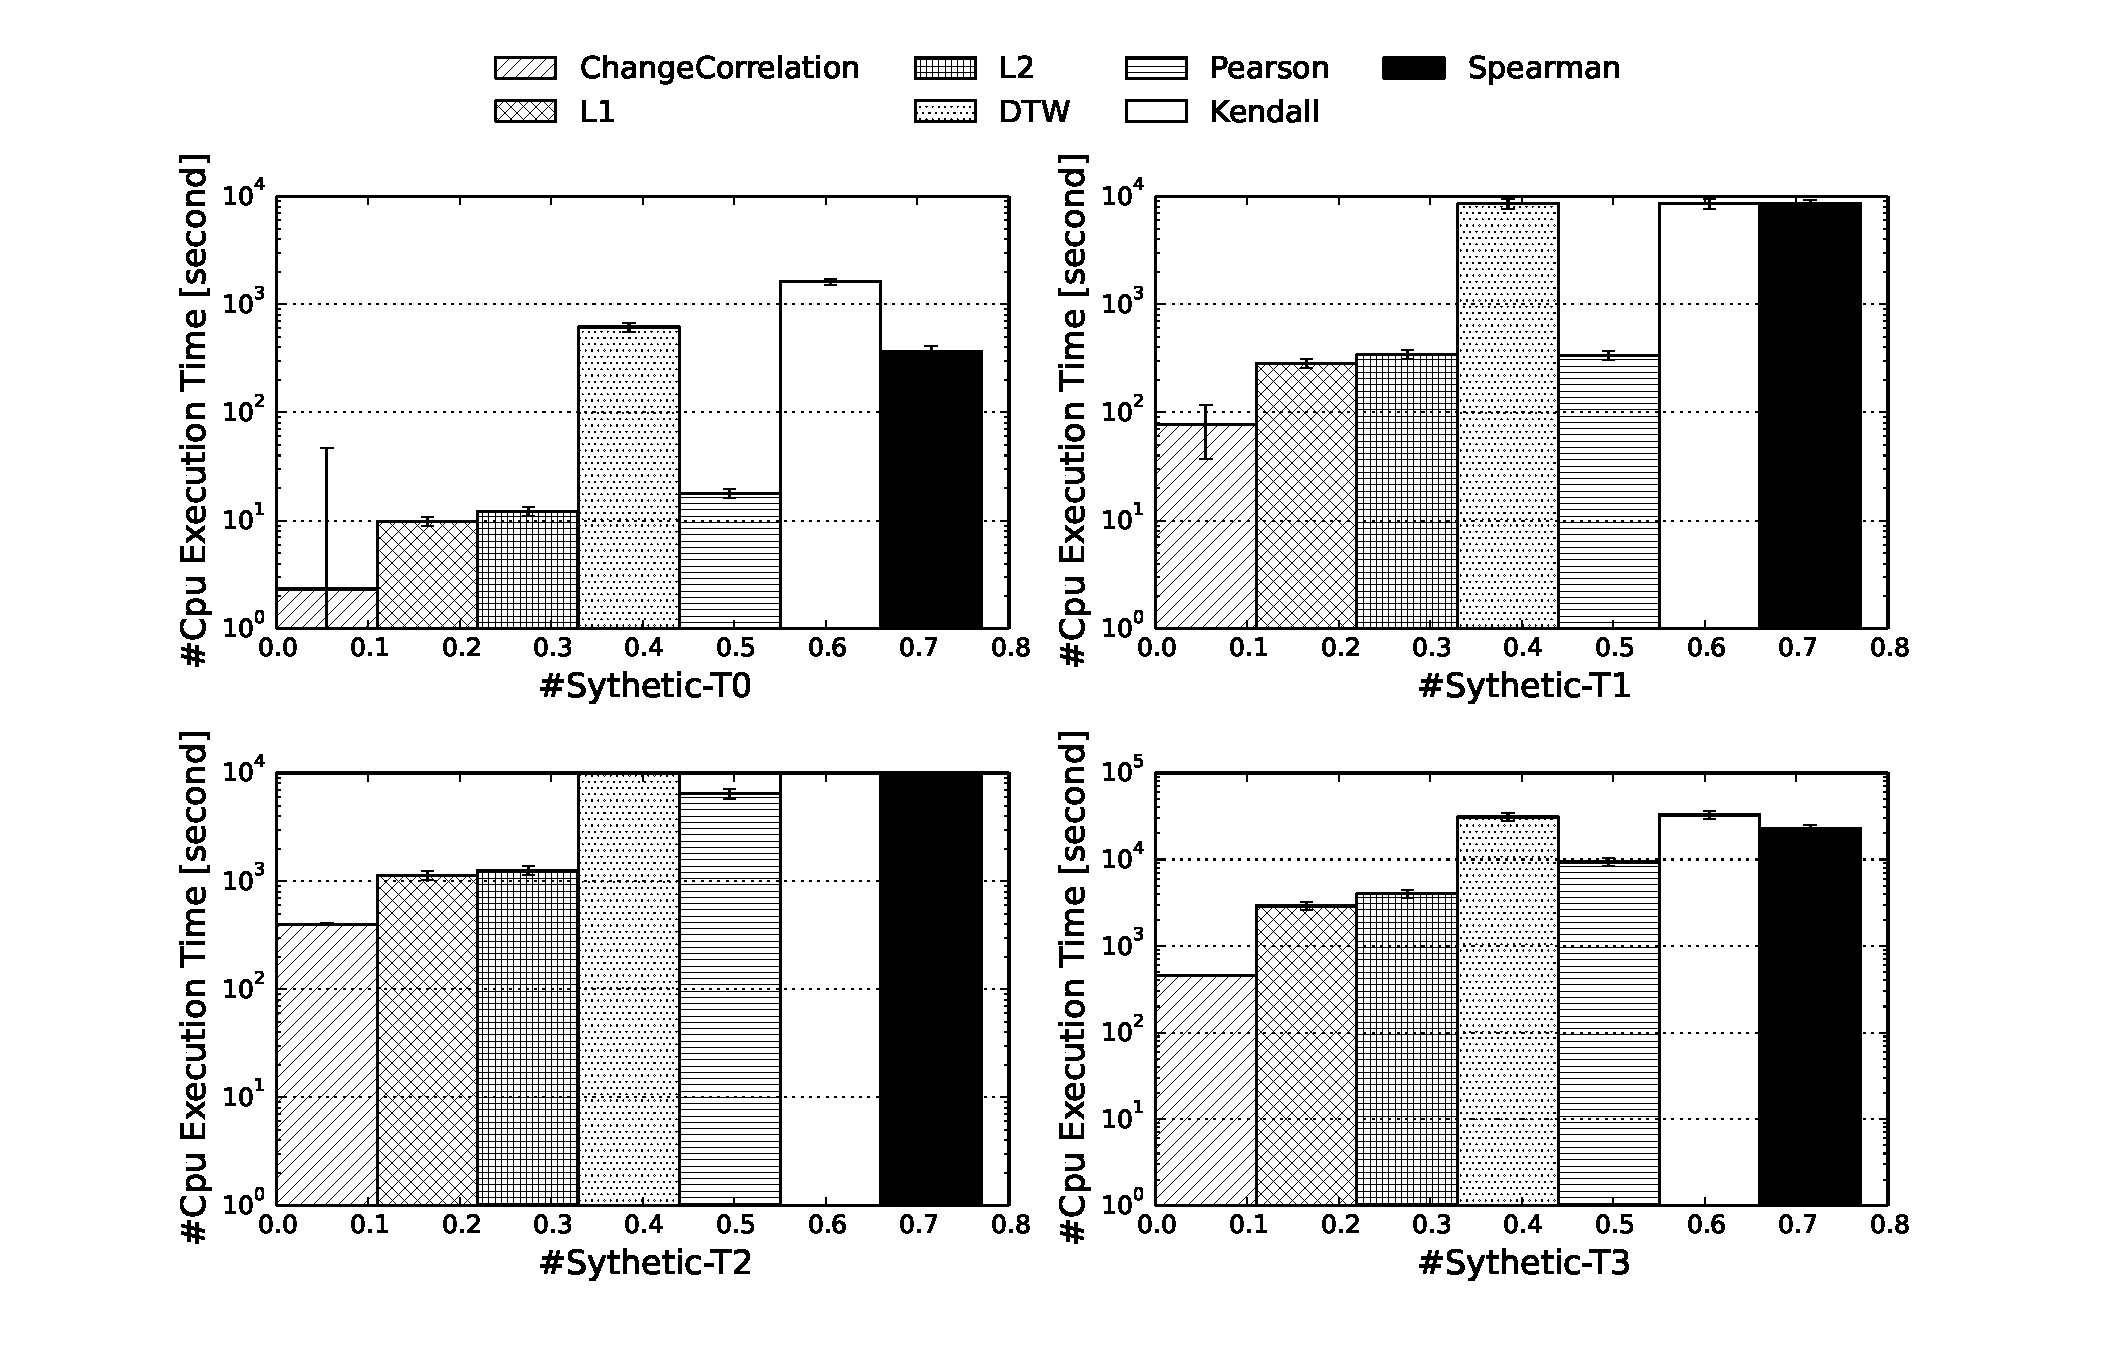
\includegraphics[width=0.8\textwidth]{SythClusPerf.eps}
\caption{Top-k Nearest Neighbor Search}
\label{Fig:ClusPerf}
\end{figure*}

\begin{figure*}[t]
\centering

\subfigure{%
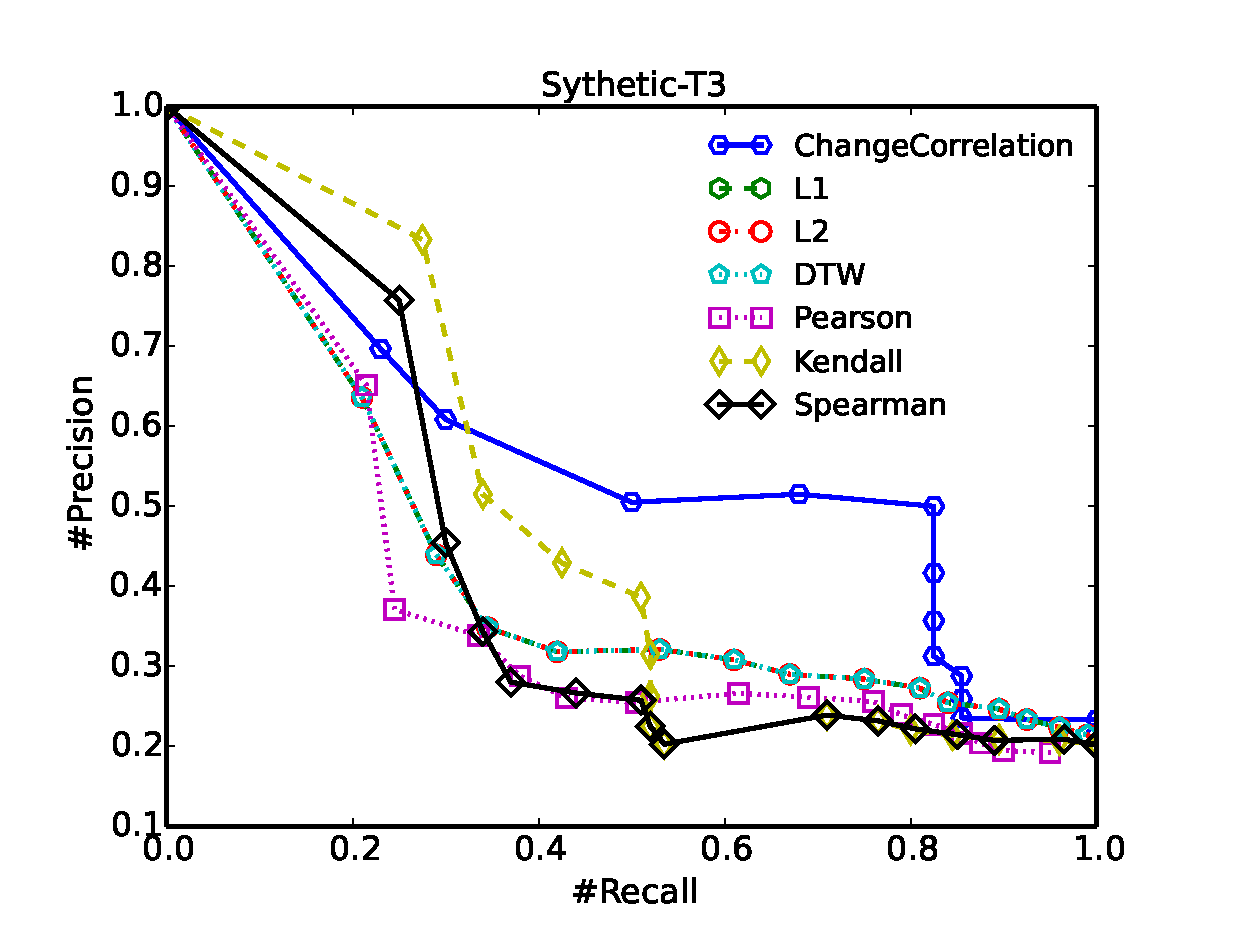
\includegraphics[width=0.41\textwidth]{PRC3.eps}
}\hspace{0.001em}
\subfigure{%
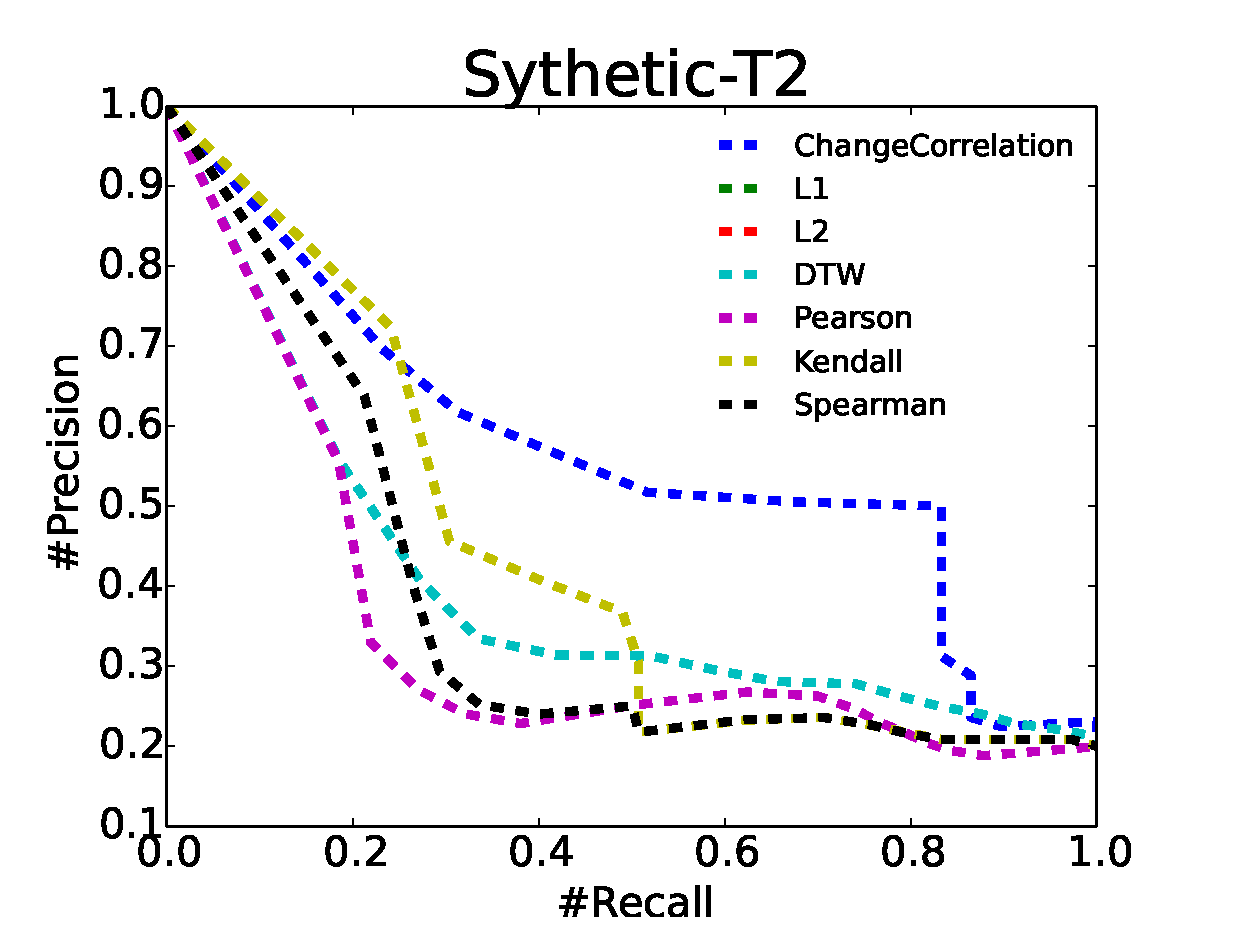
\includegraphics[width=0.41\textwidth]{PRC2.eps}
}\hspace{0.001em}
\subfigure{%
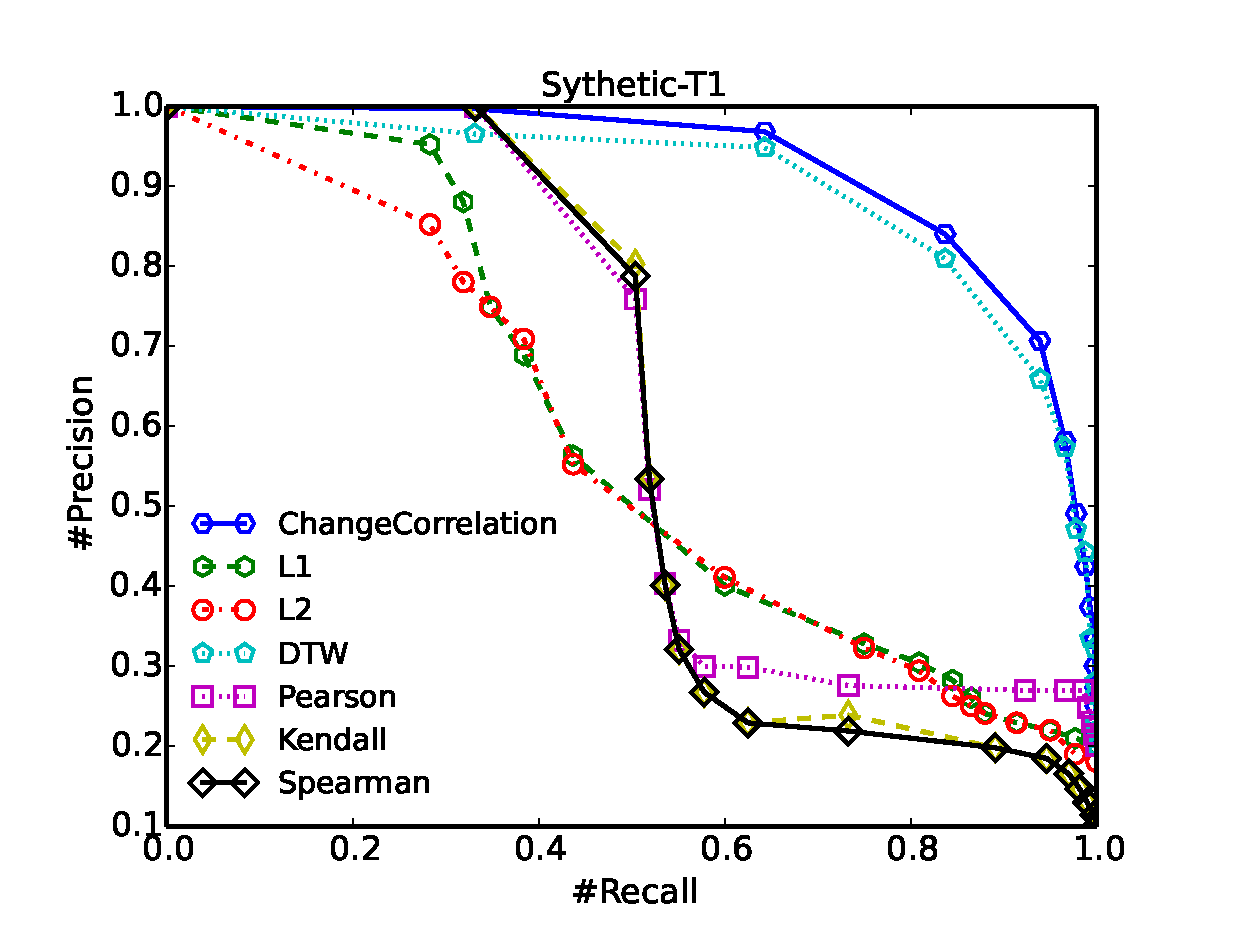
\includegraphics[width=0.41\textwidth]{PRC1.eps}
}\hspace{0.001em}
\subfigure{%
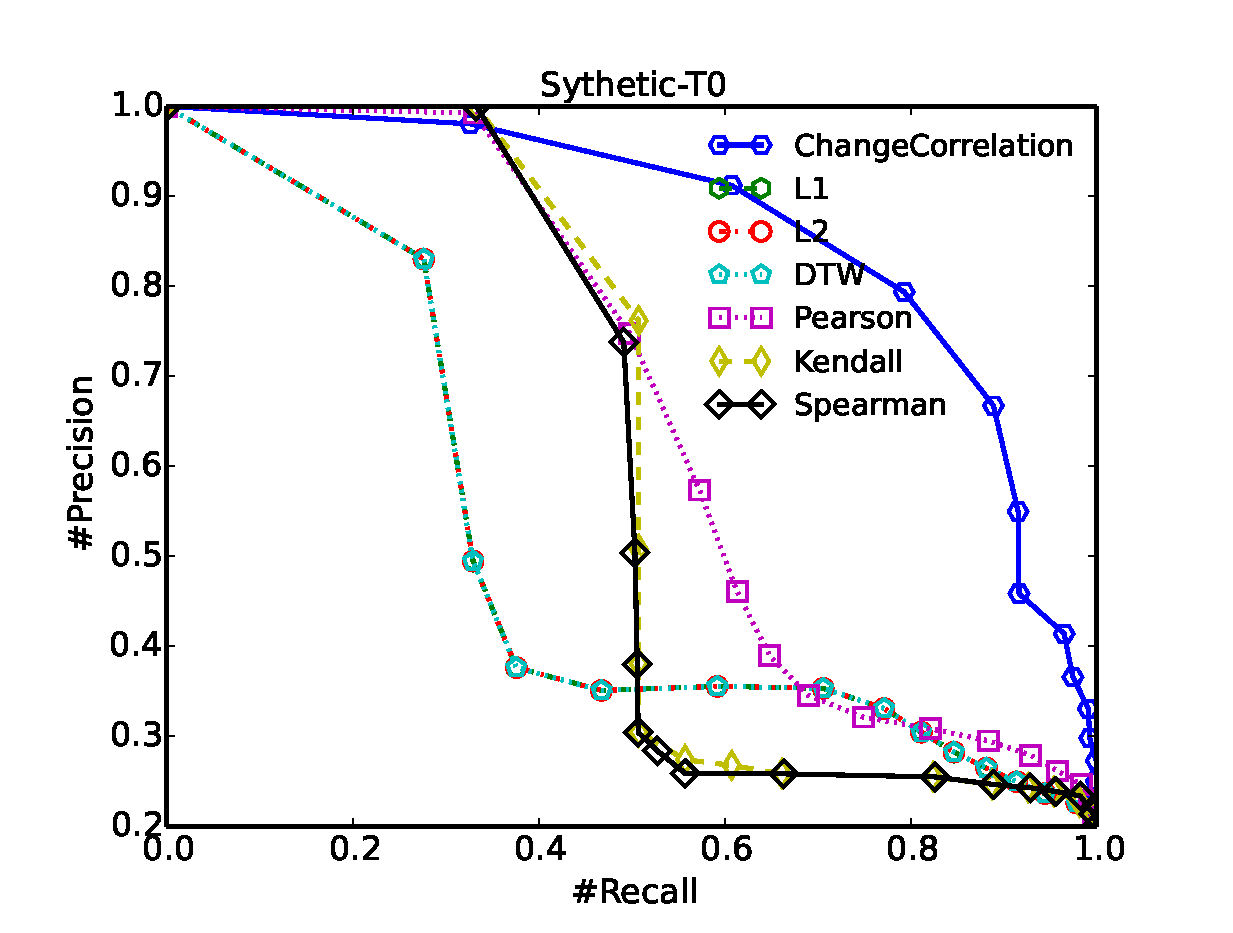
\includegraphics[width=0.41\textwidth]{PRC0.eps}
}
%
\caption{Precision Recall Curve for Different Algorithms}
\label{fig:NNPreRe}
\end{figure*}


\begin{figure*}
\centering
\subfigure{%
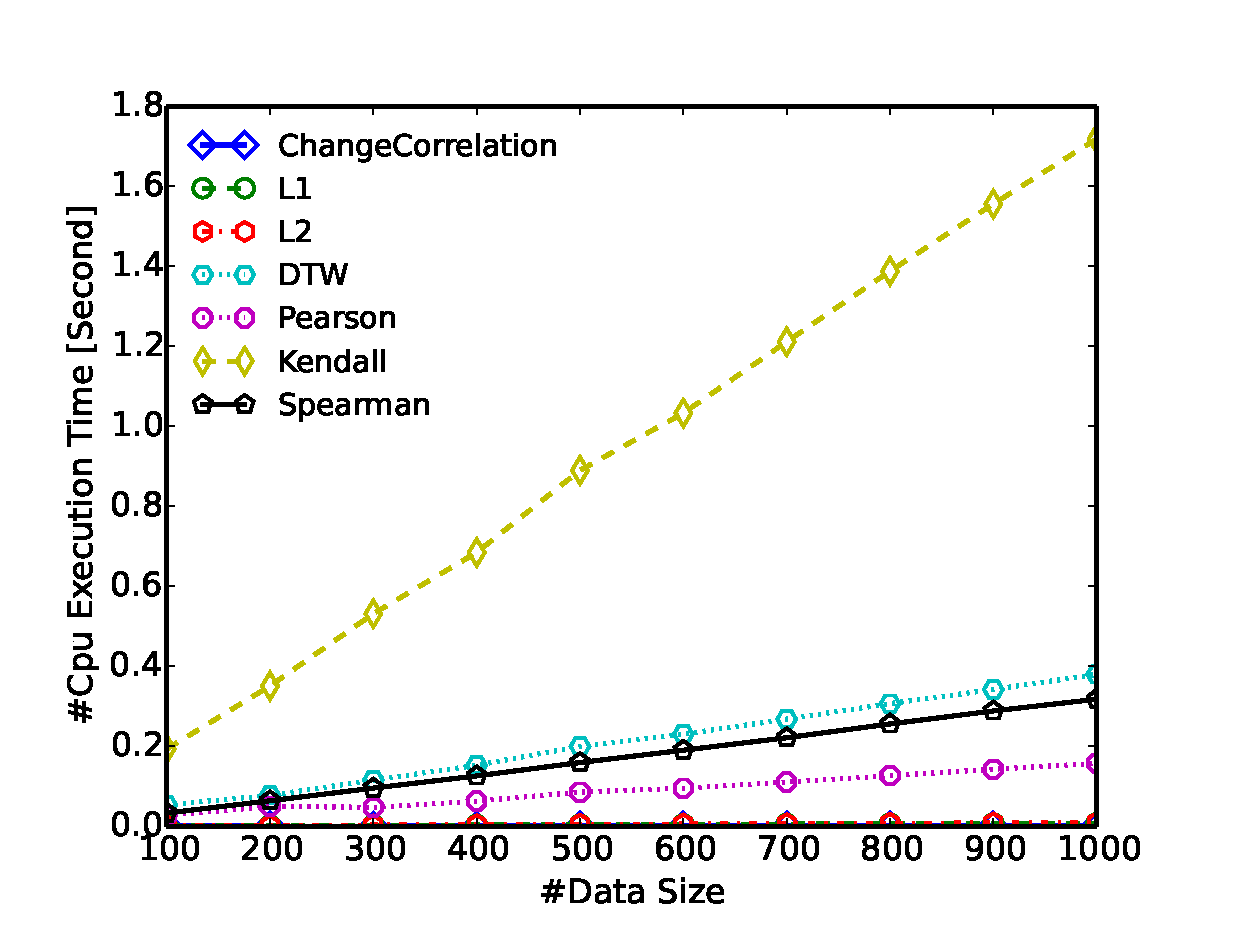
\includegraphics[width=0.45\textwidth]{VaryDataSize.eps}
}\hspace{0.001em}
\subfigure{%
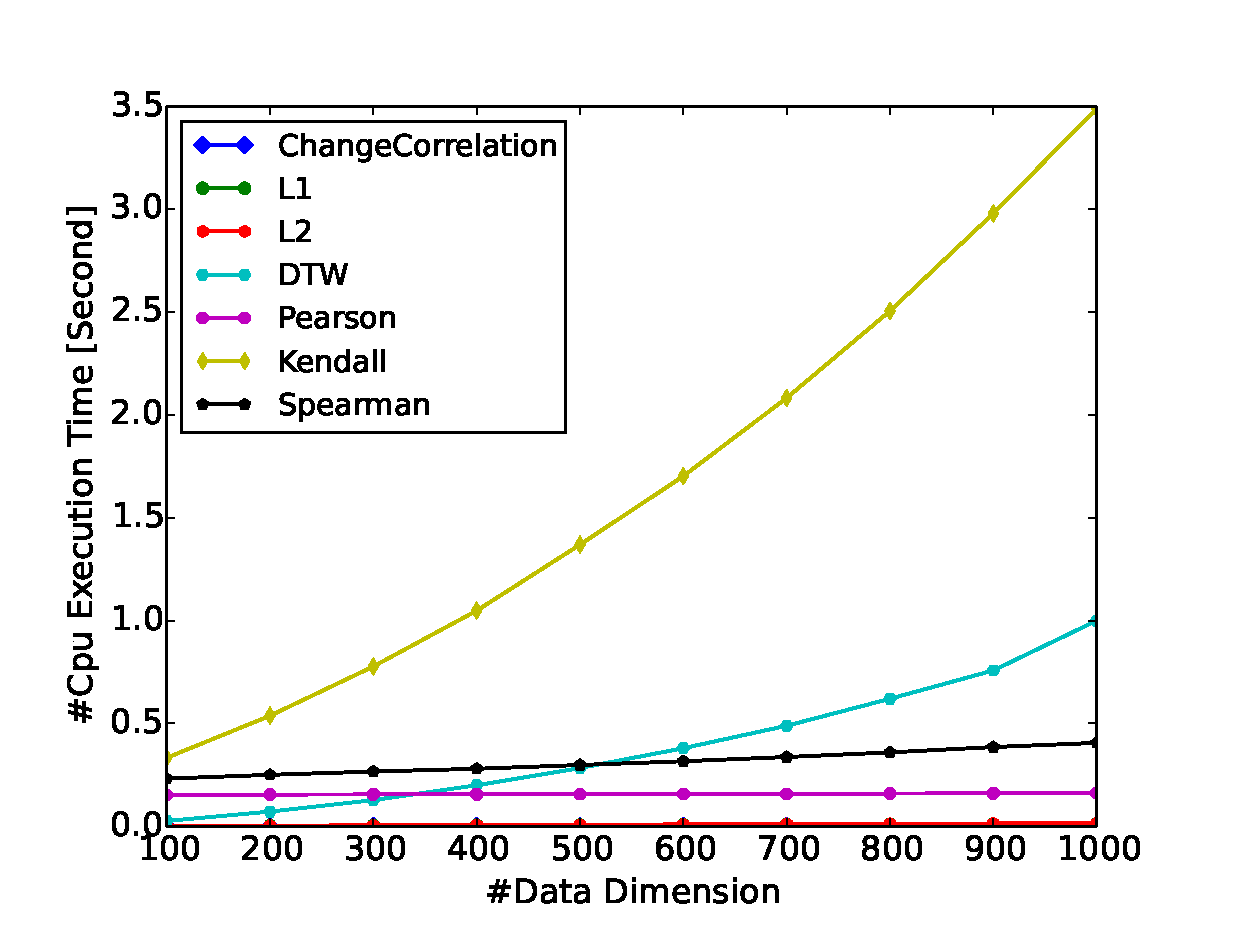
\includegraphics[width=0.45\textwidth]{VaryDataDimension.eps}
}\hspace{0.001em}
\caption{Efficiency by varying data size and dimension size}
\label{fig:NNPerf}
\end{figure*}


\subsubsection{Clustering Task}

In order to evaluate the performance of our correlation coefficient, we design a clustering task on the Synthetic Time series data. In this experiment, we only use the Hierarchical Clustering \cite{han2011data} to evaluate the performance. Because Hierarchical Clustering is very sensitive to the distance measure used, it is good for evaluating the distance measure.

Two evaluation methods are used for testing the clustering result: Accuracy \cite{han2011data}, which is calculated as the percentage of target objects clustered into the correct clusters; and Normalized Mutual Information (NMI) \cite{han2011data}, which is one of the most popular evaluation methods to evaluate the quality of clustering results.

From Table.\ref{Tab:ClusRes}, we can see that, for the change correlation coefficient, the clustering result performance is better for the high dimensional data set.
This is because that for high dimensional time series data, the proposed coefficient can extract more change information from the time series data and also make more accurate evaluation of the correlation. 
From this point of view, change based correlation is more suitable for the high dimensional time series data set.
On the other hand, Change based correlation can obtain more accuracy results in different dataset compared with both the similarity method and the correlation coefficient. So, the result of clustering show the effectiveness of our coefficient.

Fig.\ref{Fig:ClusPerf} shows the Execution time of the clustering task on each data set. From the result, we can see that change based correlation performed much faster than other algorithms. This is because, we only calculate the correlation on the extracted change information (Bit-stream), the calculating of change based correlation measure can be much faster than other similarity and correlation methods.


\subsubsection{Top-K Searching Task}

We compute precision and recall \cite{powers2011evaluation} on the data-set using the LSH-based method. And for other distance measure, we use the naive Top-K searching method. 

For precision and recall, if the Searched time series is in the same cluster of the query time series, we regard it as a relevant items, and vice verse. We range the $K$ from $1$ to the cluster size. 

For each top-k Nearest Neighbors search, the precision can be calculated as follow:

\begin{equation}
Precision =\frac{relevant~item}{K} 
\end{equation}

and the recall can be calculated as follow:

\begin{equation}
Precision =\frac{relevant~item}{Relevant~Cluster~Size} 
\end{equation}

The plots for all the three datasets are shown in Figure.\ref{fig:NNPreRe}.
We can clearly see that our proposed Change-based Correlation method gives significantly higher precision recall curves than other similarity and correlation methods. In addition the results are consistent across datasets.

Fig.\ref{fig:NNPerf} shows the execution time by vary the data size and the time series length.
In left one of Fig.\ref{fig:NNPerf}, we fix the value of time series length, and
vary the data size n. We can see that the CPU execution
time of other similarity methods increased sharply by enlarging the data size. 
And, the change based correlation do not change so much by enlarge the data size.

In right of Fig. \ref{fig:NNPerf}, we fix the size of data size, and vary the value of time series length. Based on the results, we can see that the running time of the proposed change based method with LSH doesn't so much with the increase of time series length, while other methods increase by enlarging the time series length.

\subsection{Effectiveness Study on Real Datasets}

In this section, we will compare the proposed algorithm with the baseline algorithms on two real data sets.

\subsubsection{Electrocardiogram Data set}

The first real world dataset is ECG (Electrocardiogram) time series data set. This data set comes from the the UCR time series Data set Archive \cite{UCRArchive}. We choose four ECG data set there as showed in Table. \ref{Tab:ECGData}. And the ground truth comes from the UCR data set itself.

For the clustering task, we use the Hierarchical Clustering \cite{han2011data} to evaluate the performance as before. 
From Table.\ref{Tab:ECGClus}, we can see that, for the change based correlation can obtain more accuracy results in these four ECG data set compared with both the similarity method and the correlation coefficient. So, the result of clustering show the effectiveness of our coefficient.

For the Top-K searching task. The plots for all the four ECG dataset datasets are shown in Figure.\ref{fig:ECGPRC}.
We can clearly see that our proposed Change-based Correlation method gives significantly higher precision recall curves than other similarity and correlation methods. In addition the results are consistent across datasets. This demonstrate the effectiveness of change-based correlation coefficient and the corresponding LSH search algorithm.

\begin{table*}[t]
\caption{Summary of the Four ECG Data Set}
\centering

\begin{tabular}{|c|c|c|c|}
\hline Data Set & \centering Data Size & Time Series Length & Class Numver\\
\hline CinC_ECG_torso & \centering 1380 & 1639 & 4\\
\hline ECGFiveDays & \centering 861 & 136 & 2\\
\hline TwoLeadECG & \centering 1139 & 82 & 2\\
\hline ECG5000 & \centering 4500 & 140 & 5\\
\hline
\end{tabular}
\label{Tab:ECGData}
\end{table*}

\begin{table*}[t]
\caption{Clustering Performance on Synthetic ECG Data Set From UCR Time Series Archive}
\centering
\renewcommand{\arraystretch}{1.2}
\begin{tabular}{ccccccccc} 
\toprule[2pt] 
%\hline
Dataset & Measure & Proposed & $L1$ & $L2$ & DTW & Pearson & Kendall & Spearman \\
\toprule[1.5pt] 
\multirow{2}*{\centering{CinC_ECG_torso}}
     & Accuracy & $\boldsymbol{.839\pm.011}$ & $.667\pm.068$ & $.557\pm.012$ & $.610\pm.061$ & $.531\pm.140$ & $.507\pm.019$ & $.504\pm.013$ \\
\cline{2-9}
     & NMI & $\boldsymbol{.489\pm.019}$ & $.236\pm.035$ & $.019\pm.023$ & $.010\pm.075$ & $.280\pm.55$ & $.150\pm.015$ & $.049\pm.012$ \\
\toprule[1.2pt] 
\multirow{2}*{\centering{EGG_5000}}
     & Accuracy & $\boldsymbol{.538\pm.025}$ & $.247\pm.026$ & $.262\pm.032$ & $.283\pm.012$ & $.240\pm.018$ & $.374\pm.067$ & $.341\pm.067$ \\
\cline{2-9}
     & NMI & $\boldsymbol{.401\pm.030}$ & $.003\pm.062$ & $.057\pm.043$ & $.064\pm.036$ & $.046\pm.084$ & $.404\pm.023$ & $.230\pm.042$ \\
\toprule[1.2pt] 
\multirow{2}*{\centering{TwoLeadECG}}
     & Accuracy & $\boldsymbol{.810\pm.029}$ & $.504\pm.066$ & $.538\pm.080$ & $.620\pm.022$ & $.528\pm.064$ & $.531\pm.052$ & $.519\pm.049$ \\
\cline{2-9}
     & NMI & $\boldsymbol{.680\pm.012}$ & $.081\pm.042$ & $.043\pm.056$ & $.137\pm.032$ & $.047\pm.064$ & $.062\pm.052$ & $.074\pm.049$ \\
\toprule[1.2pt] 
\multirow{2}*{\centering{ECGFiveDays}}
     & Accuracy & $\boldsymbol{.832\pm.077}$ & $.502\pm.028$ & $.527\pm.034$ & $.615\pm.062$ & $.506\pm.032$ & $.547\pm.032$ & $.519\pm.032$ \\
\cline{2-9}
     & NMI & $\boldsymbol{.765\pm.017}$ & $.002\pm.040$ & $.002\pm.043$ & $.361\pm.038$ & $.075\pm.032$ & $.023\pm.032$ & $.086\pm.032$ \\
\bottomrule[1.5pt] 
\end{tabular}
\label{Tab:ECGClus}
\end{table*}

\begin{figure*}[t]
\centering
\subfigure{%
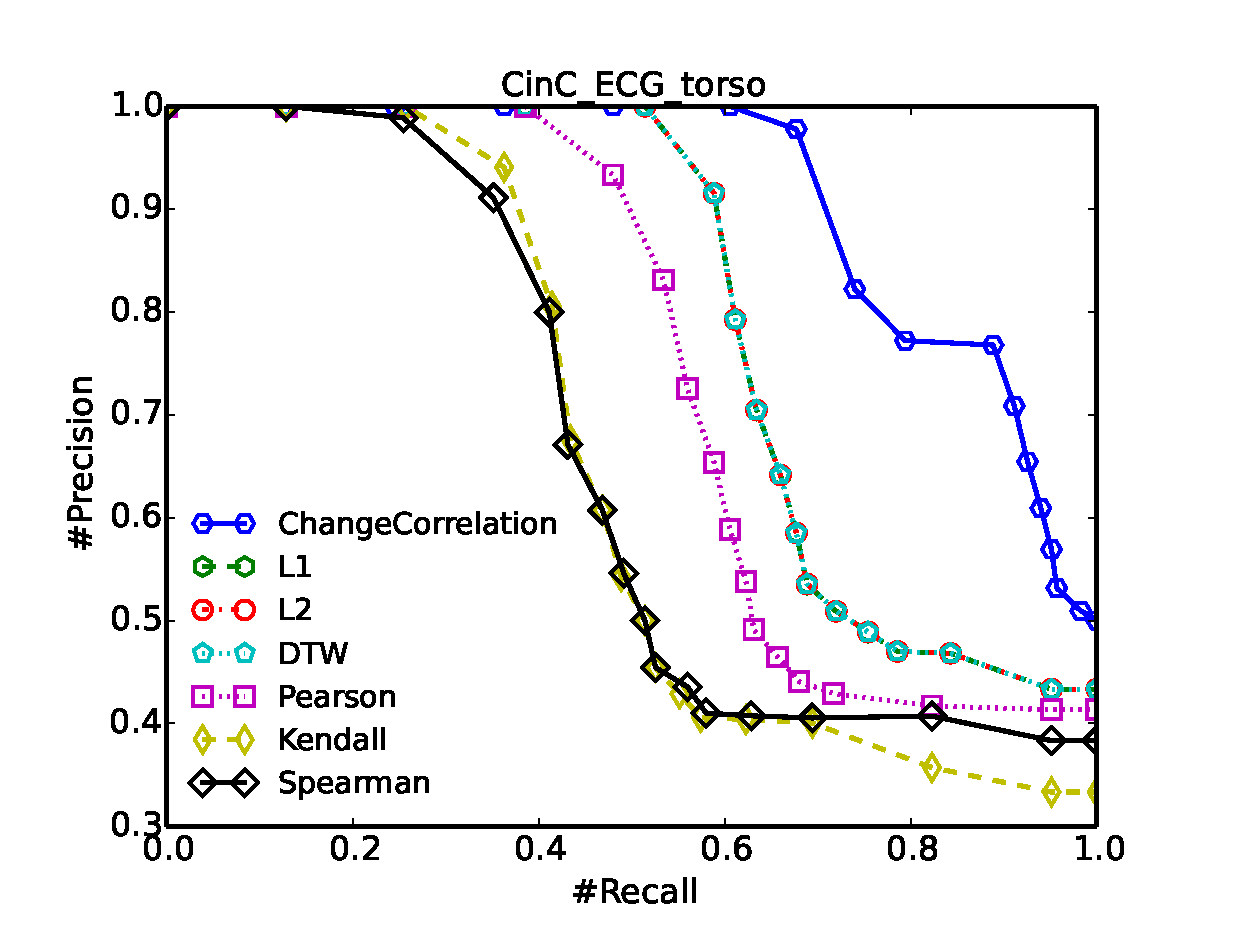
\includegraphics[width=0.45\textwidth]{PRCCinCECGtorso.eps}
}\hspace{0.001em}
\subfigure{%
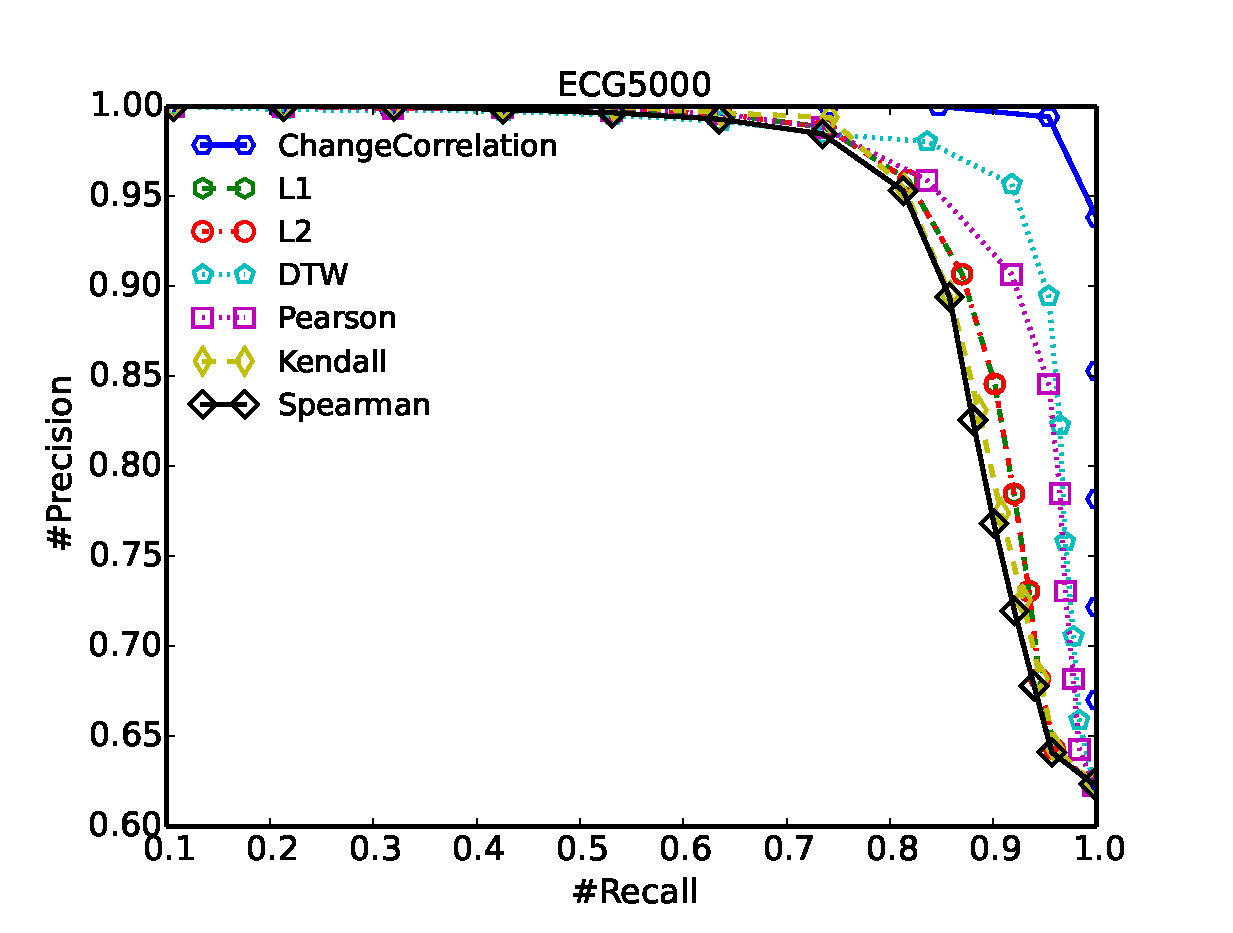
\includegraphics[width=0.45\textwidth]{PRCECG5000.eps}
}\hspace{0.001em}
\subfigure{%
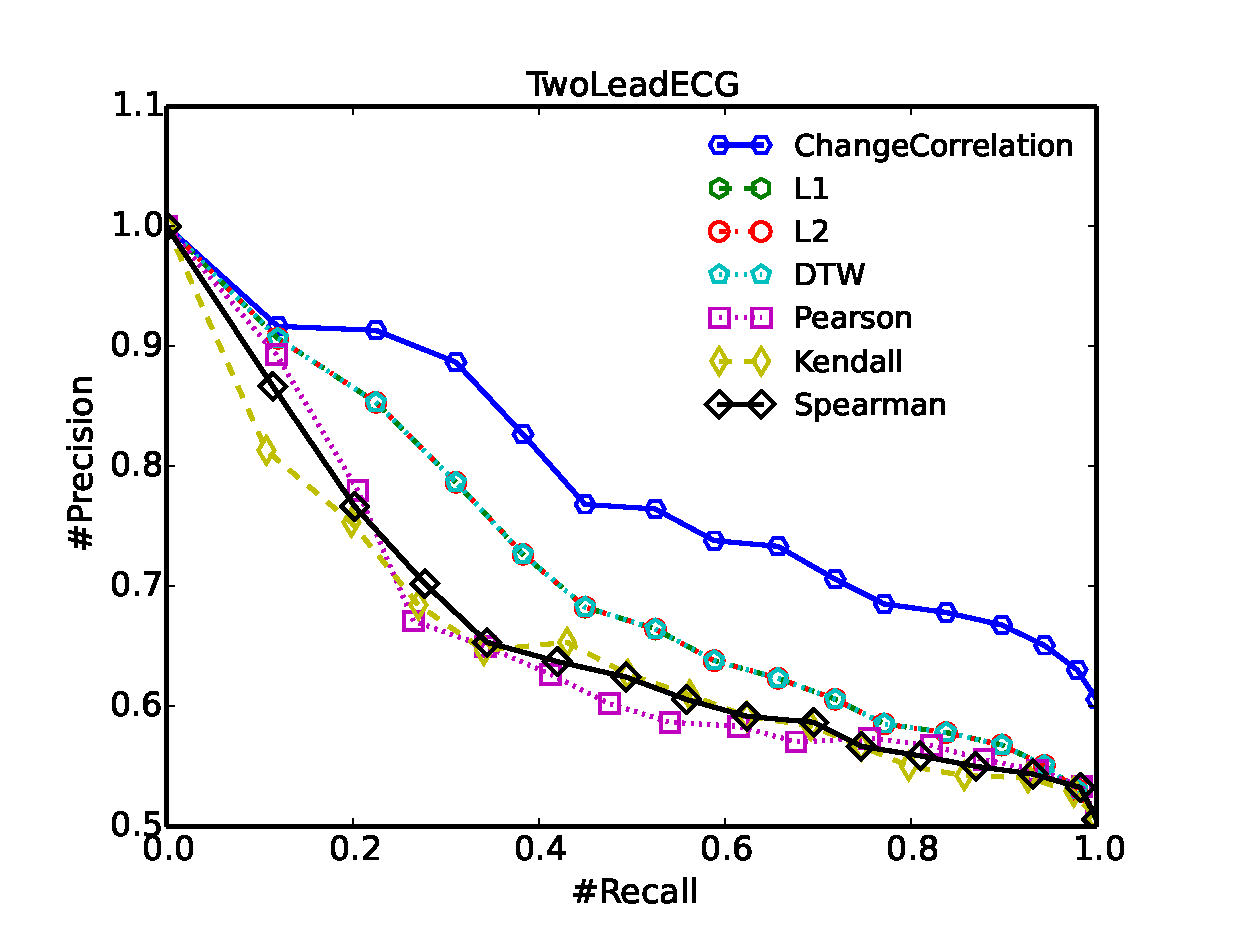
\includegraphics[width=0.45\textwidth]{PRCTwoLeadECG.eps}
}\hspace{0.001em}
\subfigure{%
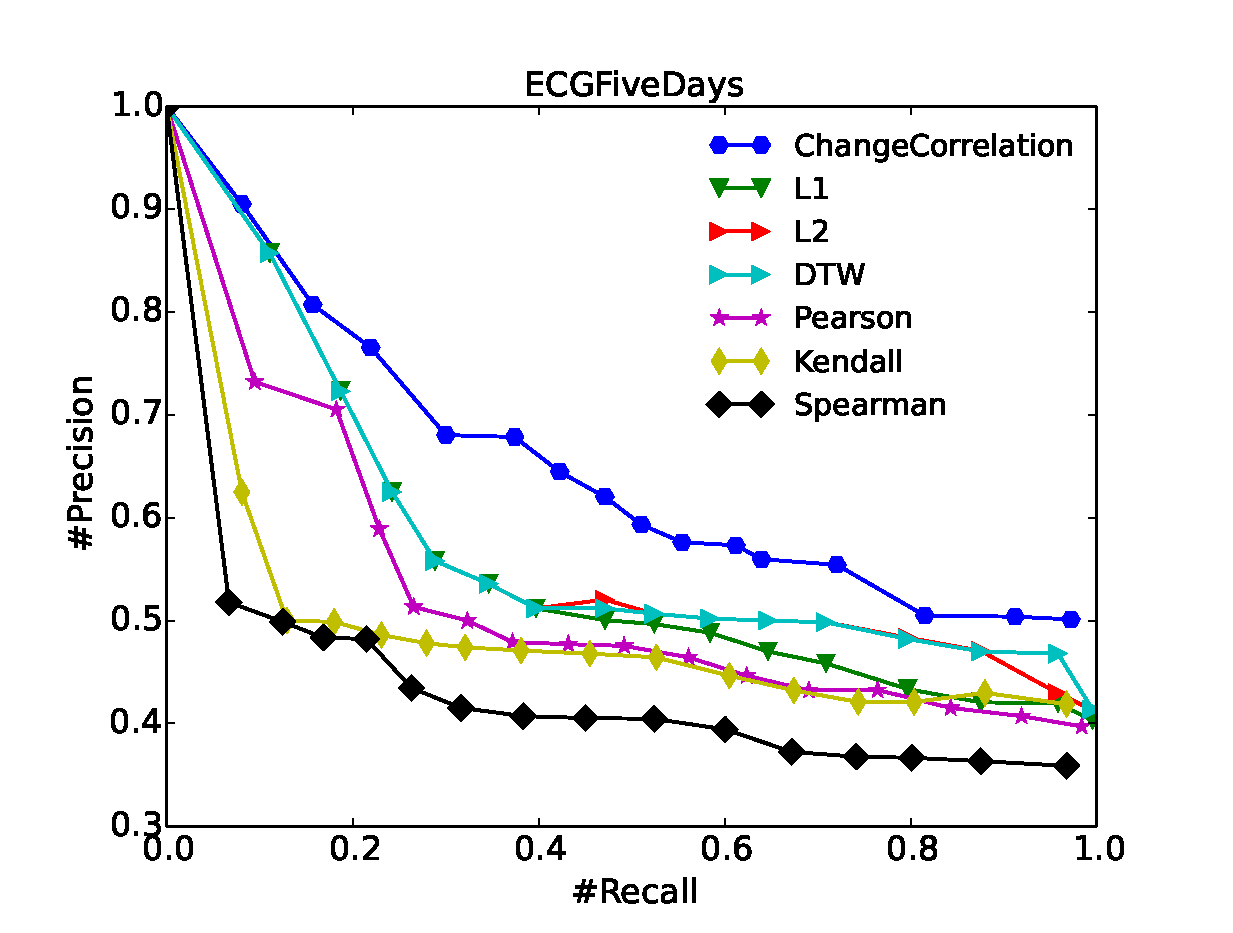
\includegraphics[width=0.45\textwidth]{PRCECGFiveDays.eps}
}\hspace{0.001em}
\caption{Precision Recall Curve (higher is better). We compare Change based correlation coefficient with other methods.}
\label{fig:ECGPRC}
\end{figure*}


\subsubsection{HPC Thread Time Series Data set}

The second real world dataset is from the HPC-tool Kit Dataset. This data set provided by HPCToolkit by analysis High performance computer during running. There are two types of thread in these two data set: main thread and other thread. So, the experiment here is based on the ground truth of two different class of thread.

We also use the Hierarchical Clustering \cite{han2011data} to evaluate the performance as before. 
From Table.\ref{Tab:HPCClus}, we can see that, for the change based correlation can obtain more accuracy results in the two HPC Thread Time series data set compared with both the similarity method and the correlation coefficient. While we can see that DTW method can also get high accuracy, this because in data set, most of the thread in same class often in same state. However, as we said before, in some cases, thread in same class, the state can be different.

The precision recall curve for the HPC Thread TIme Series data is showed in Figure \ref{fig:HPCPRC}. We can clearly see that our proposed Change-based Correlation method gives higher precision recall curves than other similarity and correlation methods. Also, DTW method can get good result too. In addition the results are consistent across datasets. This demonstrate the effectiveness of change-based correlation coefficient and the corresponding LSH search algorithm.

\begin{table}
\caption{Summary of the HPC Time Series Data Set}
\centering

\begin{tabular}{|c|c|c|}
\hline Data Set & \centering Data Size & Time Series Length \\
\hline Single PC & \centering 24 & 4096 \\
\hline MADNESS & \centering 264 & 32768 \\
\hline
\end{tabular}
\label{Tab:HPCData}
\end{table}

\begin{table*}[t]
\caption{Clustering Performance on Synthetic ECG Data Set From UCR Time Series Archive}
\centering
\renewcommand{\arraystretch}{1.2}
\begin{tabular}{ccccccccc} 
\toprule[2pt] 
%\hline
Dataset & Measure & Proposed & $L1$ & $L2$ & DTW & Pearson & Kendall & Spearman \\
\toprule[1.5pt] 
\multirow{2}*{\centering{Single PC}}
     & Accuracy & $\boldsymbol{.917\pm.011}$ & $.835\pm.068$ & $.815\pm.012$ & $.870\pm.061$ & $.501\pm.140$ & $.527\pm.019$ & $.514\pm.013$ \\
\cline{2-9}
     & NMI & $\boldsymbol{.889\pm.019}$ & $.736\pm.035$ & $.719\pm.023$ & $.860\pm.075$ & $.380\pm.55$ & $.350\pm.015$ & $.349\pm.012$ \\
\toprule[1.2pt] 
\multirow{2}*{\centering{MADNESS}}
     & Accuracy & $\boldsymbol{.938\pm.025}$ & $.927\pm.026$ & $.922\pm.032$ & $.935\pm.012$ & $.457\pm.018$ & $.474\pm.067$ & $.541\pm.067$ \\
\cline{2-9}
     & NMI & $\boldsymbol{.861\pm.030}$ & $.853\pm.062$ & $.857\pm.043$ & $.864\pm.036$ & $.346\pm.084$ & $.404\pm.423$ & $.230\pm.442$ \\
\toprule[1.2pt] 
\end{tabular}
\label{Tab:HPCClus}
\end{table*}

\begin{figure}[t]
\centering
\subfigure{%
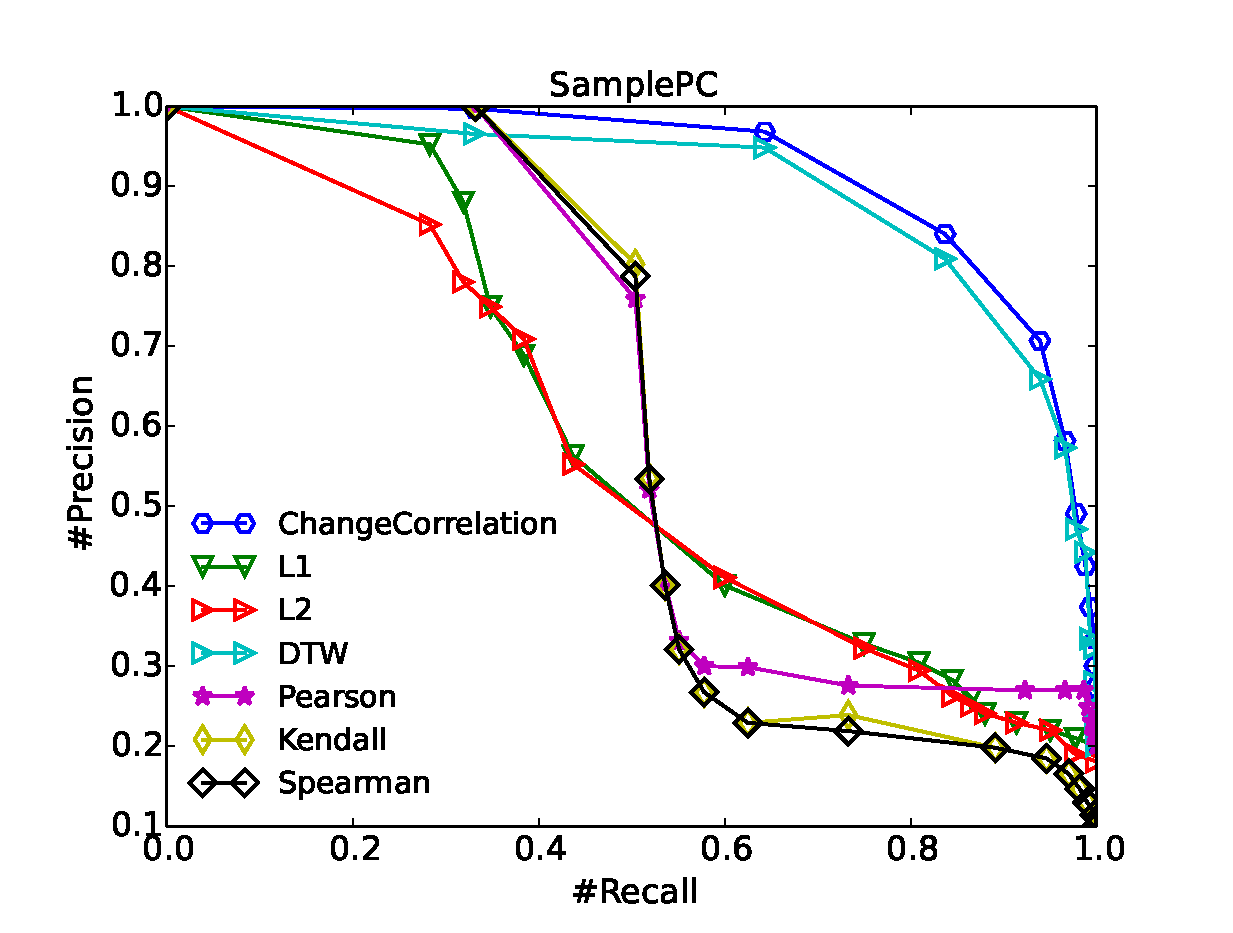
\includegraphics[width=0.45\textwidth]{PRCSamplePC.eps}
}\hspace{0.001em}
\subfigure{%
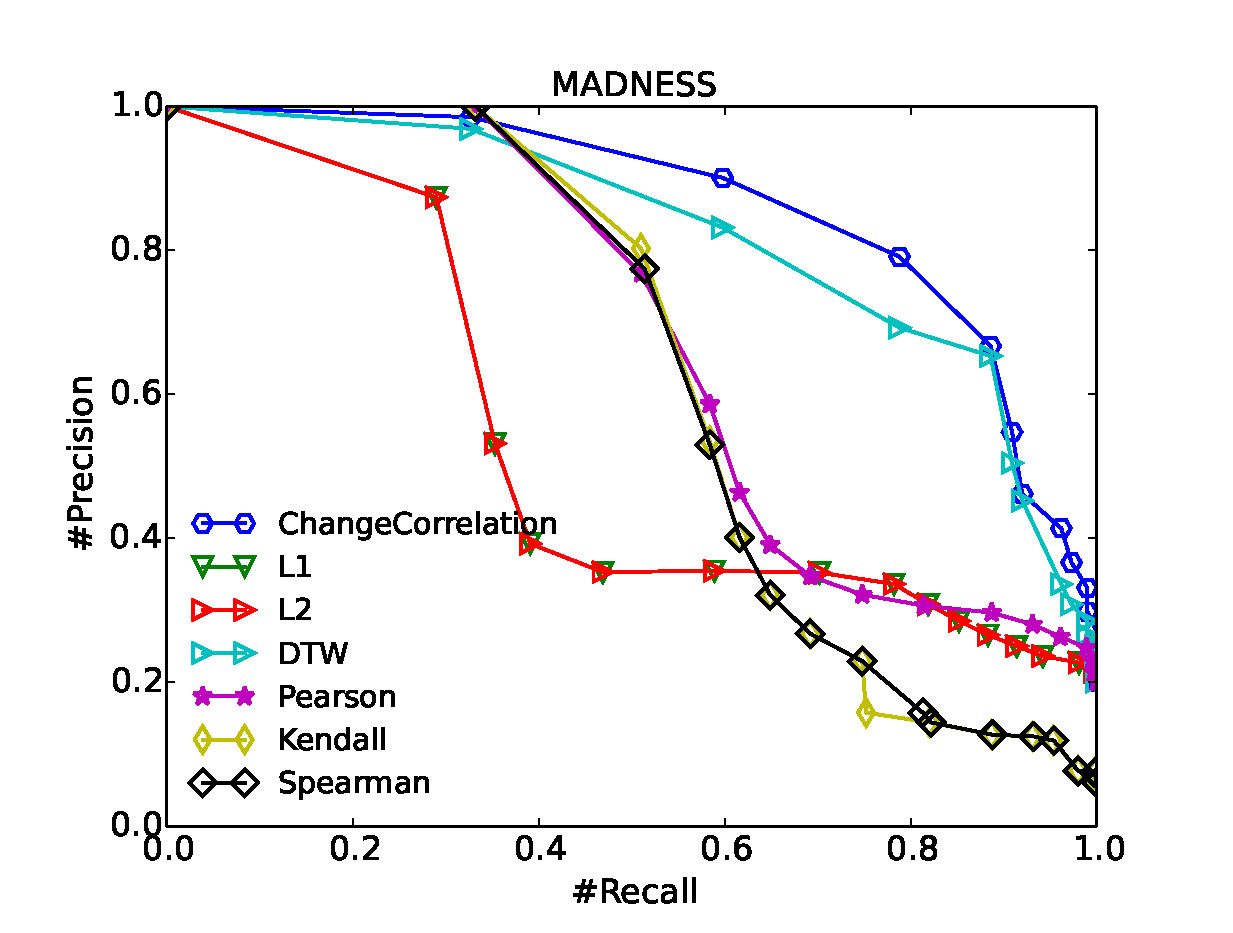
\includegraphics[width=0.45\textwidth]{PRCMADNESS.eps}
}\hspace{0.001em}
\caption{Precision Recall Curve (higher is better). We compare Change based correlation coefficient with other methods.}
\label{fig:HPCPRC}
\end{figure}





\section{Related Work}
\label{sec:relatedwork}
In this section, we brief introduce some related works of our research.

\subsection{Correlation between Time Series Data}
Correlation between two time series has been widely studied, and some of them have been included in text books~\cite{johnson2002applied}. Pearson Correlation \cite{nagelkerke1991note} is a basic correlation measure between time series, which has been widely used in practice~\cite{Zhu:VLDB:2002}. Some extensions of Pearson correlation are also widely used. For example, lagged correlation is an extension to correlate a lagged dataset with another unlagged dataset using the Pearson product-moment method. In \cite{wu2010detecting}, the author uses the lagged-correlation to estimate the lead relationship between a set of time series. Because Pearson correlation is sensitive outliers in data set, Spearman Rank correlation and Kendall Rank correlation have been used in some scenarios~\cite{Lehman:SAS:2005} to overcome the drawbacks of Pearson correlation. In Spearman correlation, data is first sorted and each value assigned a rank, e.g., 1 is assigned to the lowest value. Spearman Rank correlation is calculated by taking the Pearson product-moment correlation of the ranks of the datasets. Kendall correlation is used to measure the similarity of the orderings of the data when ranked by each of data values. Because there is no ordering relationship among the different events, the above rank based algorithms cannot be directly used in our scenario.

\subsection{Change Point Detection}

The problem of change detection has been studied for a long time, and various methods such as CUSUM (cumulated summation) \cite{basseville1993detection}, wavelet analysis \cite{kadambe1992application}, inflection point search \cite{hirano2002mining}, and Gaussian mixtures \cite{yamanishi2002unifying} have been proposed. These algorithms can be used in our method. However, our provided method can quickly detect the boolean problem of whether there is a change in the time period. We do not need to find the time series change point very accurate.

\section{Conclusion and Future Works}

\balance 

\bibliographystyle{abbrv}

\bibliography{TimeSeriesHashing}

\balance 

\end{document}
